\documentclass[aspectratio=169]{beamer}

% Default packages
\usepackage[T1]{fontenc}
\usepackage[english]{babel}
\usepackage{csquotes}
\usepackage{pgfplots}
\pgfplotsset{compat=newest}
\usepackage{booktabs}
\usepackage{siunitx}
\usepackage{amsmath}
\usepackage[backend=bibtex,style=authoryear]{biblatex}
\usepackage[ruled]{algorithm2e}
\bibliography{bibliography.bib}

% Removes icon in bibliography
\setbeamertemplate{bibliography item}{}

% Font selection
% Latin Modern
\usepackage{lmodern}
% Verdana font type
%\usepackage{verdana}
% Helvetica
%\usepackage{helvet}
% Times (text and math)
%\usepackage{newtx, newtxmath}
% Nice font combination
%\usepackage{mathptmx} % math
%\usepackage{sourcesanspro} % sans-serif
\usepackage{charter} % serif

%Avoid shaded in RMarkdown
\usepackage{color}
\usepackage{fancyvrb}
\newcommand{\VerbBar}{|}
\newcommand{\VERB}{\Verb[commandchars=\\\{\}]}
\DefineVerbatimEnvironment{Highlighting}{Verbatim}{commandchars=\\\{\}}
% Add ',fontsize=\small' for more characters per line
\usepackage{framed}
\definecolor{shadecolor}{RGB}{248,248,248}
\newenvironment{Shaded}{\begin{snugshade}}{\end{snugshade}}
\newcommand{\AlertTok}[1]{\textcolor[rgb]{0.94,0.16,0.16}{#1}}
\newcommand{\AnnotationTok}[1]{\textcolor[rgb]{0.56,0.35,0.01}{\textbf{\textit{#1}}}}
\newcommand{\AttributeTok}[1]{\textcolor[rgb]{0.77,0.63,0.00}{#1}}
\newcommand{\BaseNTok}[1]{\textcolor[rgb]{0.00,0.00,0.81}{#1}}
\newcommand{\BuiltInTok}[1]{#1}
\newcommand{\CharTok}[1]{\textcolor[rgb]{0.31,0.60,0.02}{#1}}
\newcommand{\CommentTok}[1]{\textcolor[rgb]{0.56,0.35,0.01}{\textit{#1}}}
\newcommand{\CommentVarTok}[1]{\textcolor[rgb]{0.56,0.35,0.01}{\textbf{\textit{#1}}}}
\newcommand{\ConstantTok}[1]{\textcolor[rgb]{0.00,0.00,0.00}{#1}}
\newcommand{\ControlFlowTok}[1]{\textcolor[rgb]{0.13,0.29,0.53}{\textbf{#1}}}
\newcommand{\DataTypeTok}[1]{\textcolor[rgb]{0.13,0.29,0.53}{#1}}
\newcommand{\DecValTok}[1]{\textcolor[rgb]{0.00,0.00,0.81}{#1}}
\newcommand{\DocumentationTok}[1]{\textcolor[rgb]{0.56,0.35,0.01}{\textbf{\textit{#1}}}}
\newcommand{\ErrorTok}[1]{\textcolor[rgb]{0.64,0.00,0.00}{\textbf{#1}}}
\newcommand{\ExtensionTok}[1]{#1}
\newcommand{\FloatTok}[1]{\textcolor[rgb]{0.00,0.00,0.81}{#1}}
\newcommand{\FunctionTok}[1]{\textcolor[rgb]{0.00,0.00,0.00}{#1}}
\newcommand{\ImportTok}[1]{#1}
\newcommand{\InformationTok}[1]{\textcolor[rgb]{0.56,0.35,0.01}{\textbf{\textit{#1}}}}
\newcommand{\KeywordTok}[1]{\textcolor[rgb]{0.13,0.29,0.53}{\textbf{#1}}}
\newcommand{\NormalTok}[1]{#1}
\newcommand{\OperatorTok}[1]{\textcolor[rgb]{0.81,0.36,0.00}{\textbf{#1}}}
\newcommand{\OtherTok}[1]{\textcolor[rgb]{0.56,0.35,0.01}{#1}}
\newcommand{\PreprocessorTok}[1]{\textcolor[rgb]{0.56,0.35,0.01}{\textit{#1}}}
\newcommand{\RegionMarkerTok}[1]{#1}
\newcommand{\SpecialCharTok}[1]{\textcolor[rgb]{0.00,0.00,0.00}{#1}}
\newcommand{\SpecialStringTok}[1]{\textcolor[rgb]{0.31,0.60,0.02}{#1}}
\newcommand{\StringTok}[1]{\textcolor[rgb]{0.31,0.60,0.02}{#1}}
\newcommand{\VariableTok}[1]{\textcolor[rgb]{0.00,0.00,0.00}{#1}}
\newcommand{\VerbatimStringTok}[1]{\textcolor[rgb]{0.31,0.60,0.02}{#1}}
\newcommand{\WarningTok}[1]{\textcolor[rgb]{0.56,0.35,0.01}{\textbf{\textit{#1}}}}

% Use DTU theme, see below for options
\usetheme[department=compute]{DTU}

\title[Automated and Early Detection of Disease Outbreaks]{Automated and
Early Detection of Disease Outbreaks}
\author{Kasper Schou Telkamp}
\institute{Section for Dynamical Systems}
\date{2023-02-09}
	
\newcommand{\tabitem}{{\color{dtured}$\bullet$} }

\DeclareMathOperator{\E}{E}
\DeclareMathOperator{\V}{V}
\DeclareMathOperator{\G}{G}
\DeclareMathOperator{\N}{N}
\DeclareMathOperator{\NB}{NB}
\DeclareMathOperator{\Pois}{Pois}
\DeclareMathOperator{\Geom}{Geom}


\begin{document}


\frame{
	\maketitle
}

\frame{
	\frametitle{Outline}
	\tableofcontents
}

\hypertarget{data}{%
\section{Data}\label{data}}

\begin{frame}{Data}
\tiny

\begin{figure}[H]
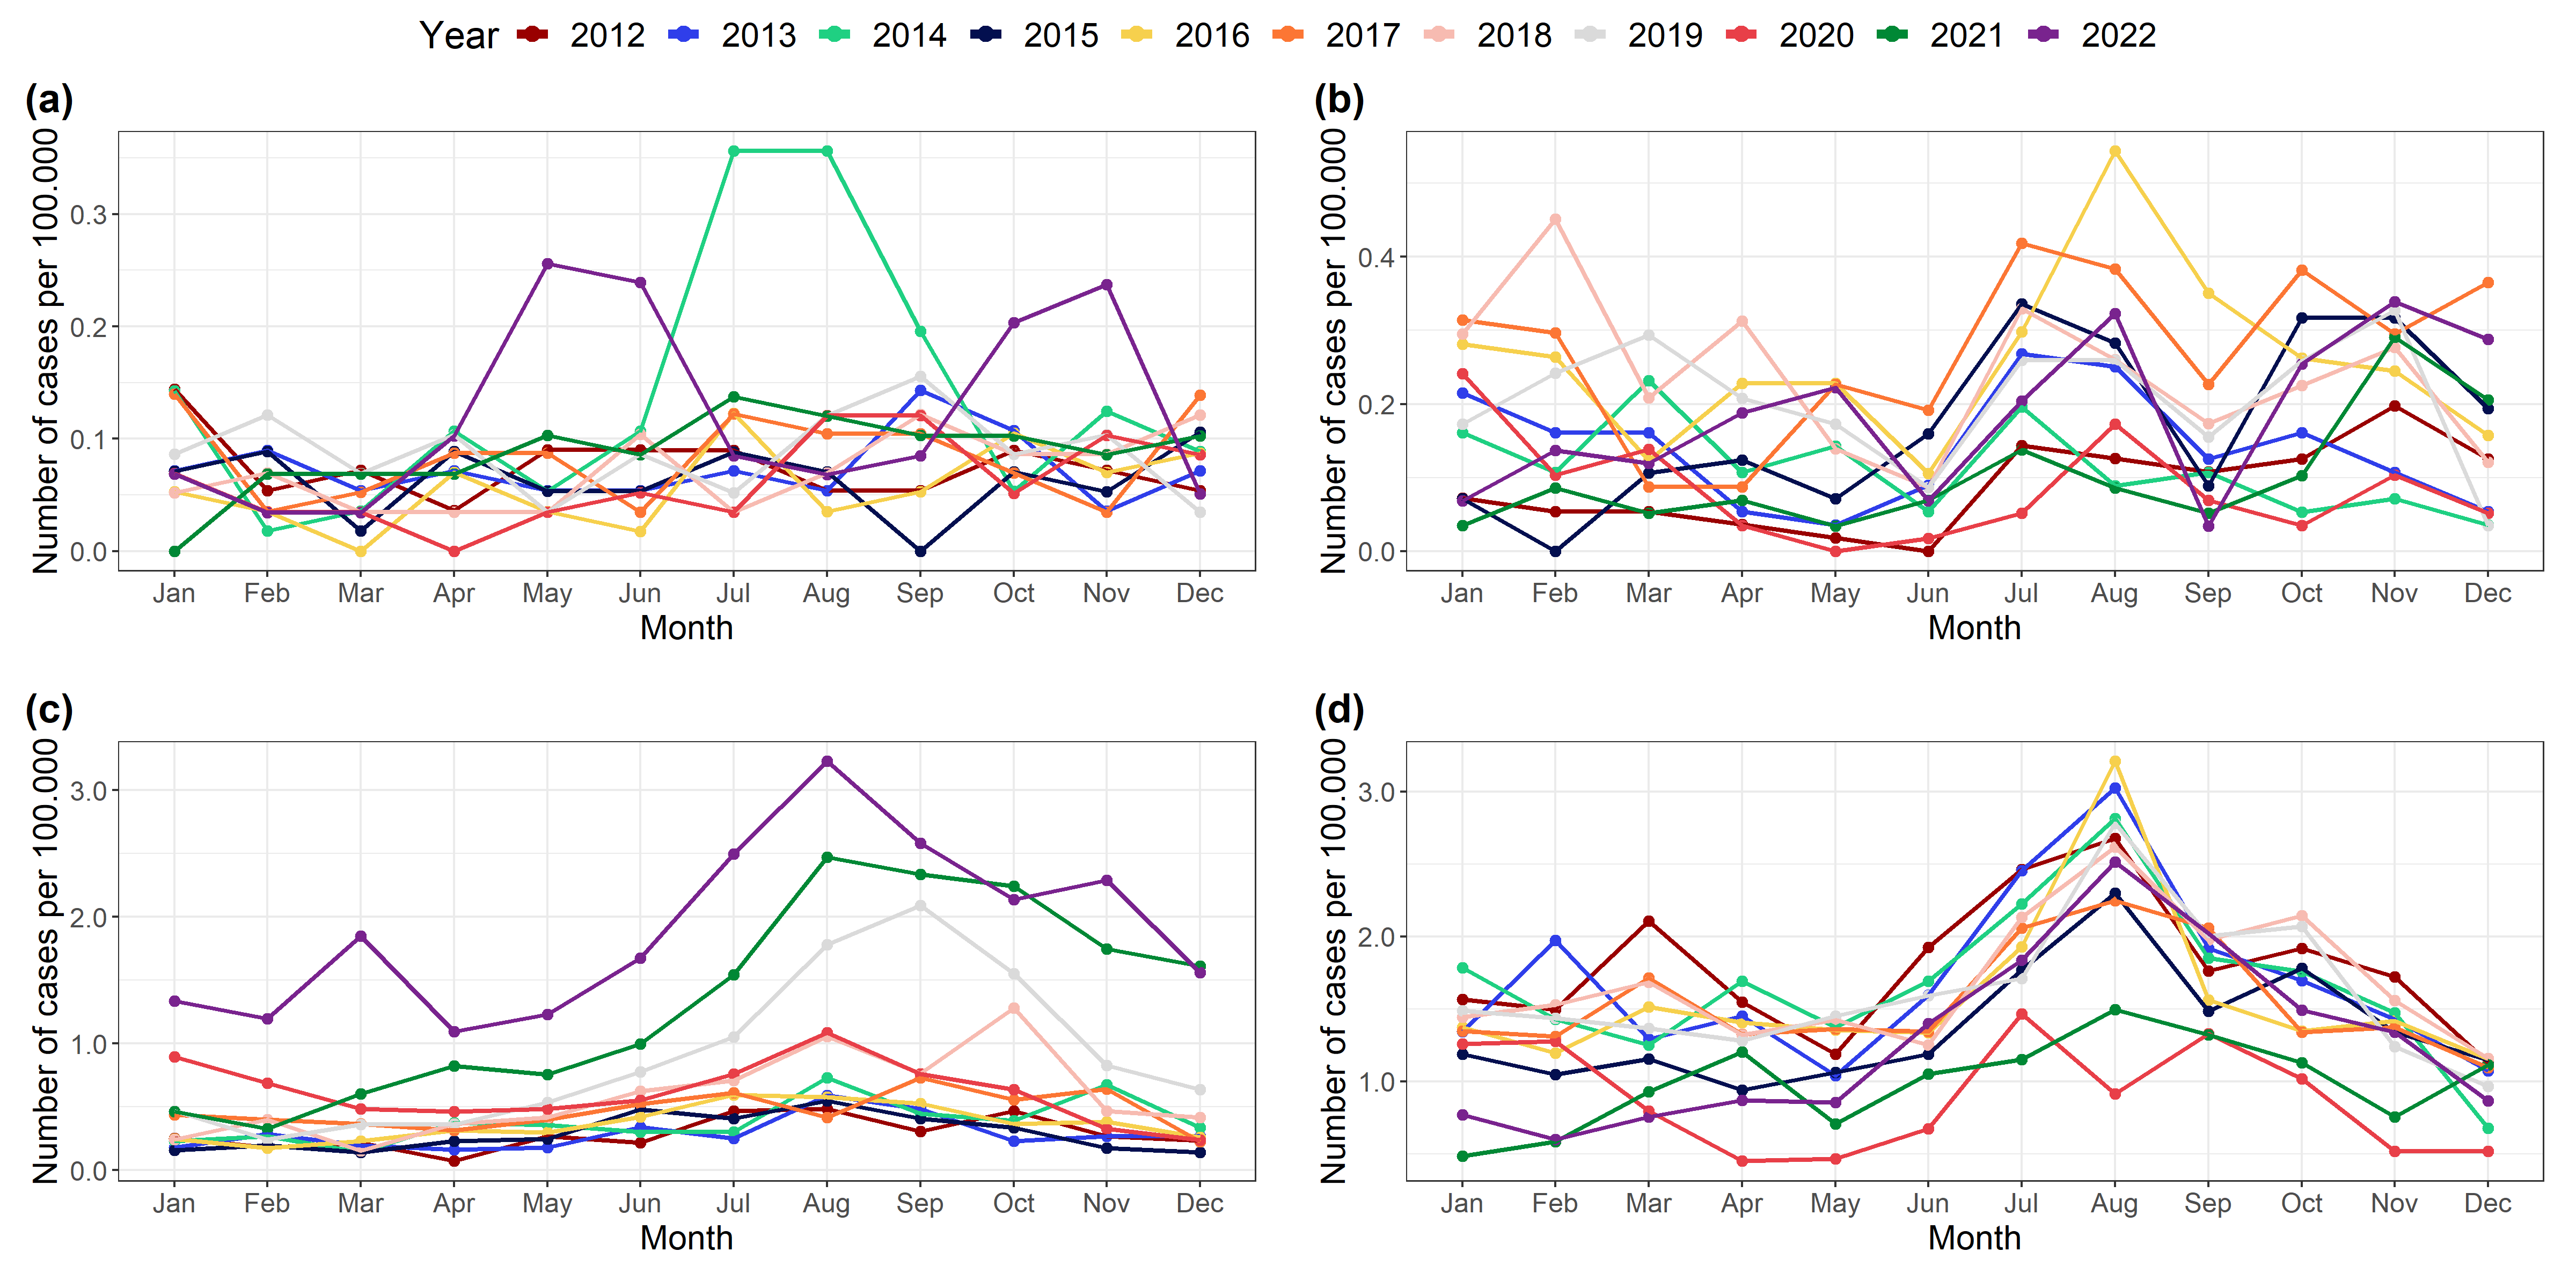
\includegraphics[width=0.8\linewidth]{../figures/EpiPlot} \caption{Epidemic curve showing the incidence per 100,000 in Denmark, 2012-2022, for the subset of diseases considered in this master thesis. (a) Listeriosis, (b) Shigellosis, (c) STEC, and (d) Salmonellosis.}\label{fig:EpiPlot}
\end{figure}

\normalsize
\end{frame}

\hypertarget{focusing-on-stec}{%
\subsection{Focusing on STEC}\label{focusing-on-stec}}

\begin{frame}{Focusing on STEC}
\tiny

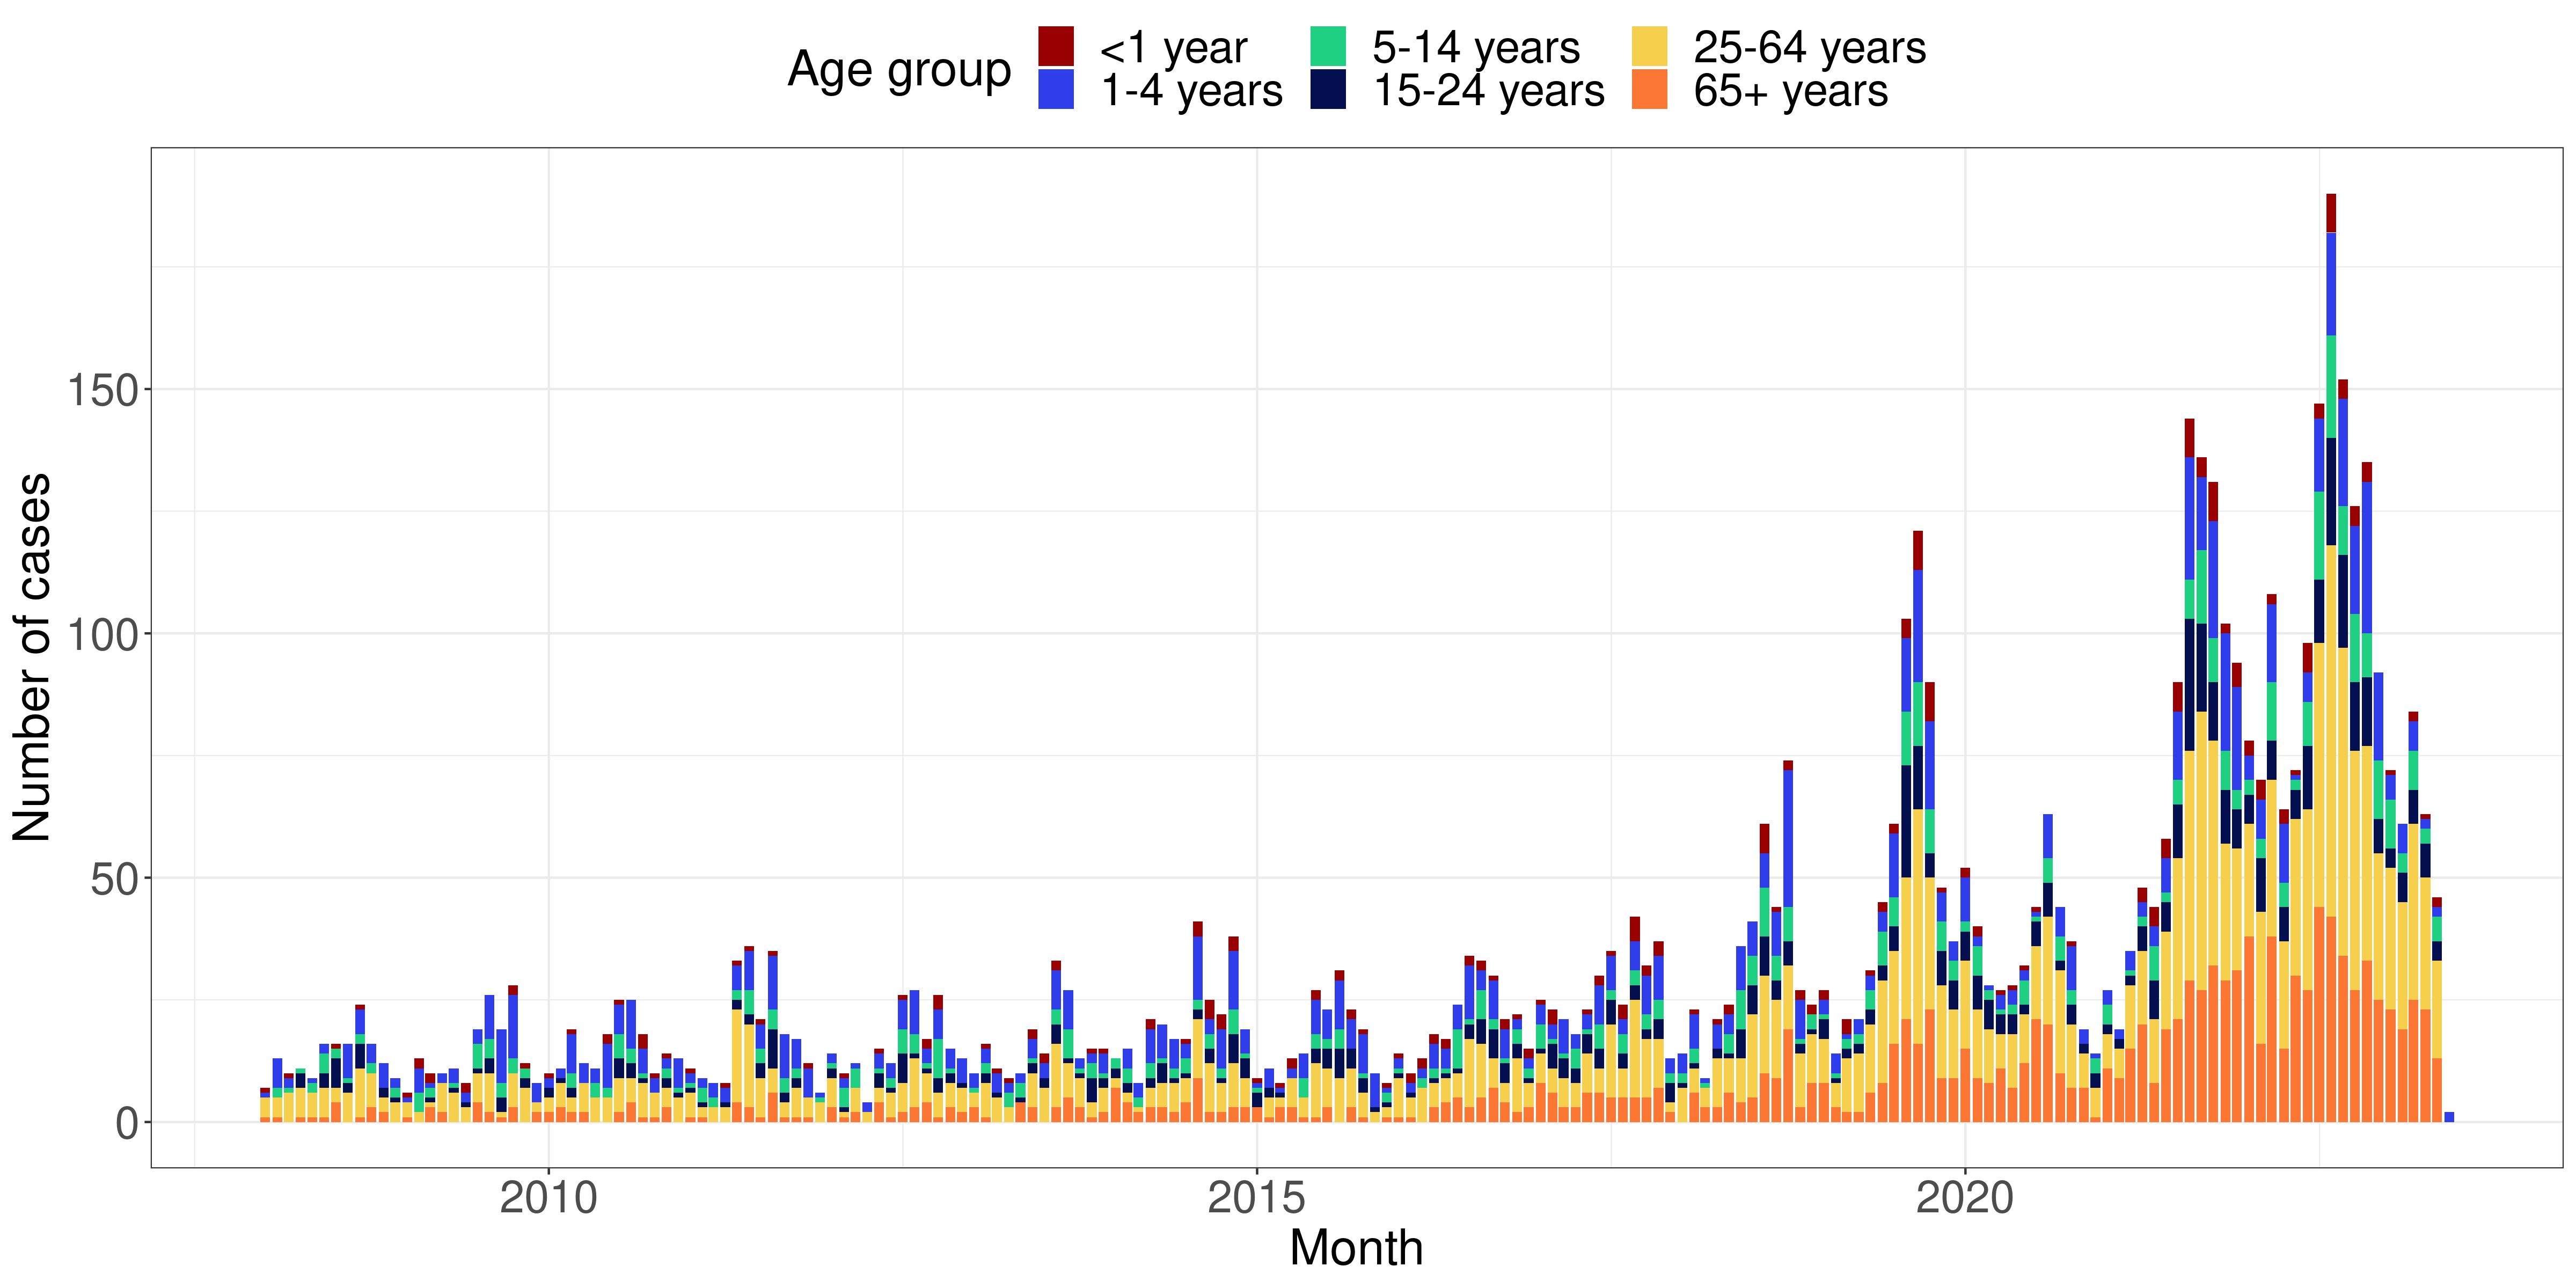
\includegraphics[width=1\linewidth]{../figures/STEC_long_plot}

\normalsize
\end{frame}

\hypertarget{novel-outbreak-detection-algorithm}{%
\section{Novel outbreak detection
algorithm}\label{novel-outbreak-detection-algorithm}}

\begin{frame}{Novel outbreak detection algorithm}
\begin{algorithm}[H]
\caption{Test}
  \KwData{This text}
  \KwResult{Hello}
  \For{$i=1$ \KwTo $T$}{
    Do something
  }
\end{algorithm}
\end{frame}

\hypertarget{model-formulas}{%
\section{Model formulas}\label{model-formulas}}

\begin{frame}{Model formulas}
\begin{equation}
  \log(\lambda_{it})=\boldsymbol{x}_{it}^T\boldsymbol{\beta}+\log(n_{it}), \quad i=1,\dots,k, \quad t=1,\dots,T
\end{equation}
\end{frame}

\hypertarget{agegroup}{%
\subsection{Agegroup}\label{agegroup}}

\begin{frame}{Agegroup}
\begin{equation}
  \log(\lambda_{it}) = \beta(ageGroup_{i}) + \log(n_{it})
\end{equation}
\end{frame}

\hypertarget{agegroup-and-seasonality}{%
\subsection{Agegroup and seasonality}\label{agegroup-and-seasonality}}

\begin{frame}{Agegroup and seasonality}
\begin{equation}
  \log(\lambda_{it}) = \beta(ageGroup_{i}) \beta_i + \sin\Big(\frac{\pi\cdot monthInYear_t}{6}\Big) \beta_{\sin} + \cos\Big(\frac{\pi \cdot monthInYear_t}{6}\Big) \beta_{\cos} + \log(n_{it})
\end{equation}
\end{frame}

\hypertarget{hierarchical-poisson-normal-model}{%
\section{Hierarchical Poisson Normal
model}\label{hierarchical-poisson-normal-model}}

\begin{frame}{Hierarchical Poisson Normal model}
\begin{subequations} \label{eq:PoisN}
  \begin{alignat}{2}
    \boldsymbol{Y|u} &\sim \Pois \big( \boldsymbol{\lambda} \exp(\boldsymbol{u}) \big) \label{eq:pois_n0} \\ 
    \boldsymbol{u} &\sim \N(\boldsymbol{0},I\sigma^2) \label{eq:pois_n1}
  \end{alignat}
\end{subequations}
\end{frame}

\hypertarget{implementation}{%
\subsection{Implementation}\label{implementation}}

\begin{frame}[fragile]{Implementation}
\tiny

\begin{Shaded}
\begin{Highlighting}[]
\PreprocessorTok{\#include }\ImportTok{\textless{}TMB.hpp\textgreater{}}\PreprocessorTok{              }\CommentTok{// Links in the TMB libraries}

\KeywordTok{template}\OperatorTok{\textless{}}\KeywordTok{class}\NormalTok{ Type}\OperatorTok{\textgreater{}}
\NormalTok{Type objective\_function}\OperatorTok{\textless{}}\NormalTok{Type}\OperatorTok{\textgreater{}::}\KeywordTok{operator}\OperatorTok{()} \OperatorTok{()}
\OperatorTok{\{}
\NormalTok{  DATA\_VECTOR}\OperatorTok{(}\NormalTok{y}\OperatorTok{);}                               \CommentTok{// Data vector transmitted from R}
\NormalTok{  DATA\_VECTOR}\OperatorTok{(}\NormalTok{x}\OperatorTok{);}                       \CommentTok{// Data vector transmitted from R}
\NormalTok{  DATA\_MATRIX}\OperatorTok{(}\NormalTok{X}\OperatorTok{);}                       \CommentTok{// Design matrix transmitted from R}
  
\NormalTok{  PARAMETER\_VECTOR}\OperatorTok{(}\NormalTok{u}\OperatorTok{);}                      \CommentTok{// Random effects}
  
  \CommentTok{// Parameters}
\NormalTok{  PARAMETER\_VECTOR}\OperatorTok{(}\NormalTok{beta}\OperatorTok{);}         \CommentTok{// Parameter value transmitted from R}
\NormalTok{  PARAMETER}\OperatorTok{(}\NormalTok{log\_sigma\_u}\OperatorTok{);}               \CommentTok{// Parameter value transmitted from R}
  
\NormalTok{  vector}\OperatorTok{\textless{}}\NormalTok{Type}\OperatorTok{\textgreater{}}\NormalTok{ lambda  }\OperatorTok{=}\NormalTok{ exp}\OperatorTok{(}\NormalTok{X}\OperatorTok{*}\NormalTok{beta}\OperatorTok{{-}}\NormalTok{log}\OperatorTok{(}\NormalTok{x}\OperatorTok{)+}\NormalTok{u}\OperatorTok{);}
\NormalTok{  Type sigma\_u }\OperatorTok{=}\NormalTok{ exp}\OperatorTok{(}\NormalTok{log\_sigma\_u}\OperatorTok{);}
  
  \DataTypeTok{int}\NormalTok{ nobs }\OperatorTok{=}\NormalTok{ y}\OperatorTok{.}\NormalTok{size}\OperatorTok{();}
\NormalTok{  Type mean\_ran }\OperatorTok{=}\NormalTok{ Type}\OperatorTok{(}\DecValTok{0}\OperatorTok{);}
  
\NormalTok{  Type f }\OperatorTok{=} \DecValTok{0}\OperatorTok{;}                           \CommentTok{// Declare the "objective function"}
  \ControlFlowTok{for}\OperatorTok{(}\DataTypeTok{int}\NormalTok{ t}\OperatorTok{=}\DecValTok{0}\OperatorTok{;}\NormalTok{ t }\OperatorTok{\textless{}}\NormalTok{ nobs}\OperatorTok{;}\NormalTok{ t}\OperatorTok{++)\{}
\NormalTok{    f }\OperatorTok{{-}=}\NormalTok{ dnorm}\OperatorTok{(}\NormalTok{u}\OperatorTok{[}\NormalTok{t}\OperatorTok{],}\NormalTok{mean\_ran}\OperatorTok{,}\NormalTok{sigma\_u}\OperatorTok{,}\KeywordTok{true}\OperatorTok{);}
\NormalTok{    f }\OperatorTok{{-}=}\NormalTok{ dpois}\OperatorTok{(}\NormalTok{y}\OperatorTok{[}\NormalTok{t}\OperatorTok{],}\NormalTok{lambda}\OperatorTok{[}\NormalTok{t}\OperatorTok{],}\KeywordTok{true}\OperatorTok{);}
  \OperatorTok{\}}
  
  \ControlFlowTok{return}\NormalTok{ f}\OperatorTok{;}
\OperatorTok{\}}
\end{Highlighting}
\end{Shaded}

\normalsize
\end{frame}

\hypertarget{results}{%
\subsection{Results}\label{results}}

\begin{frame}{Model performance}
\protect\hypertarget{model-performance}{}
\tiny

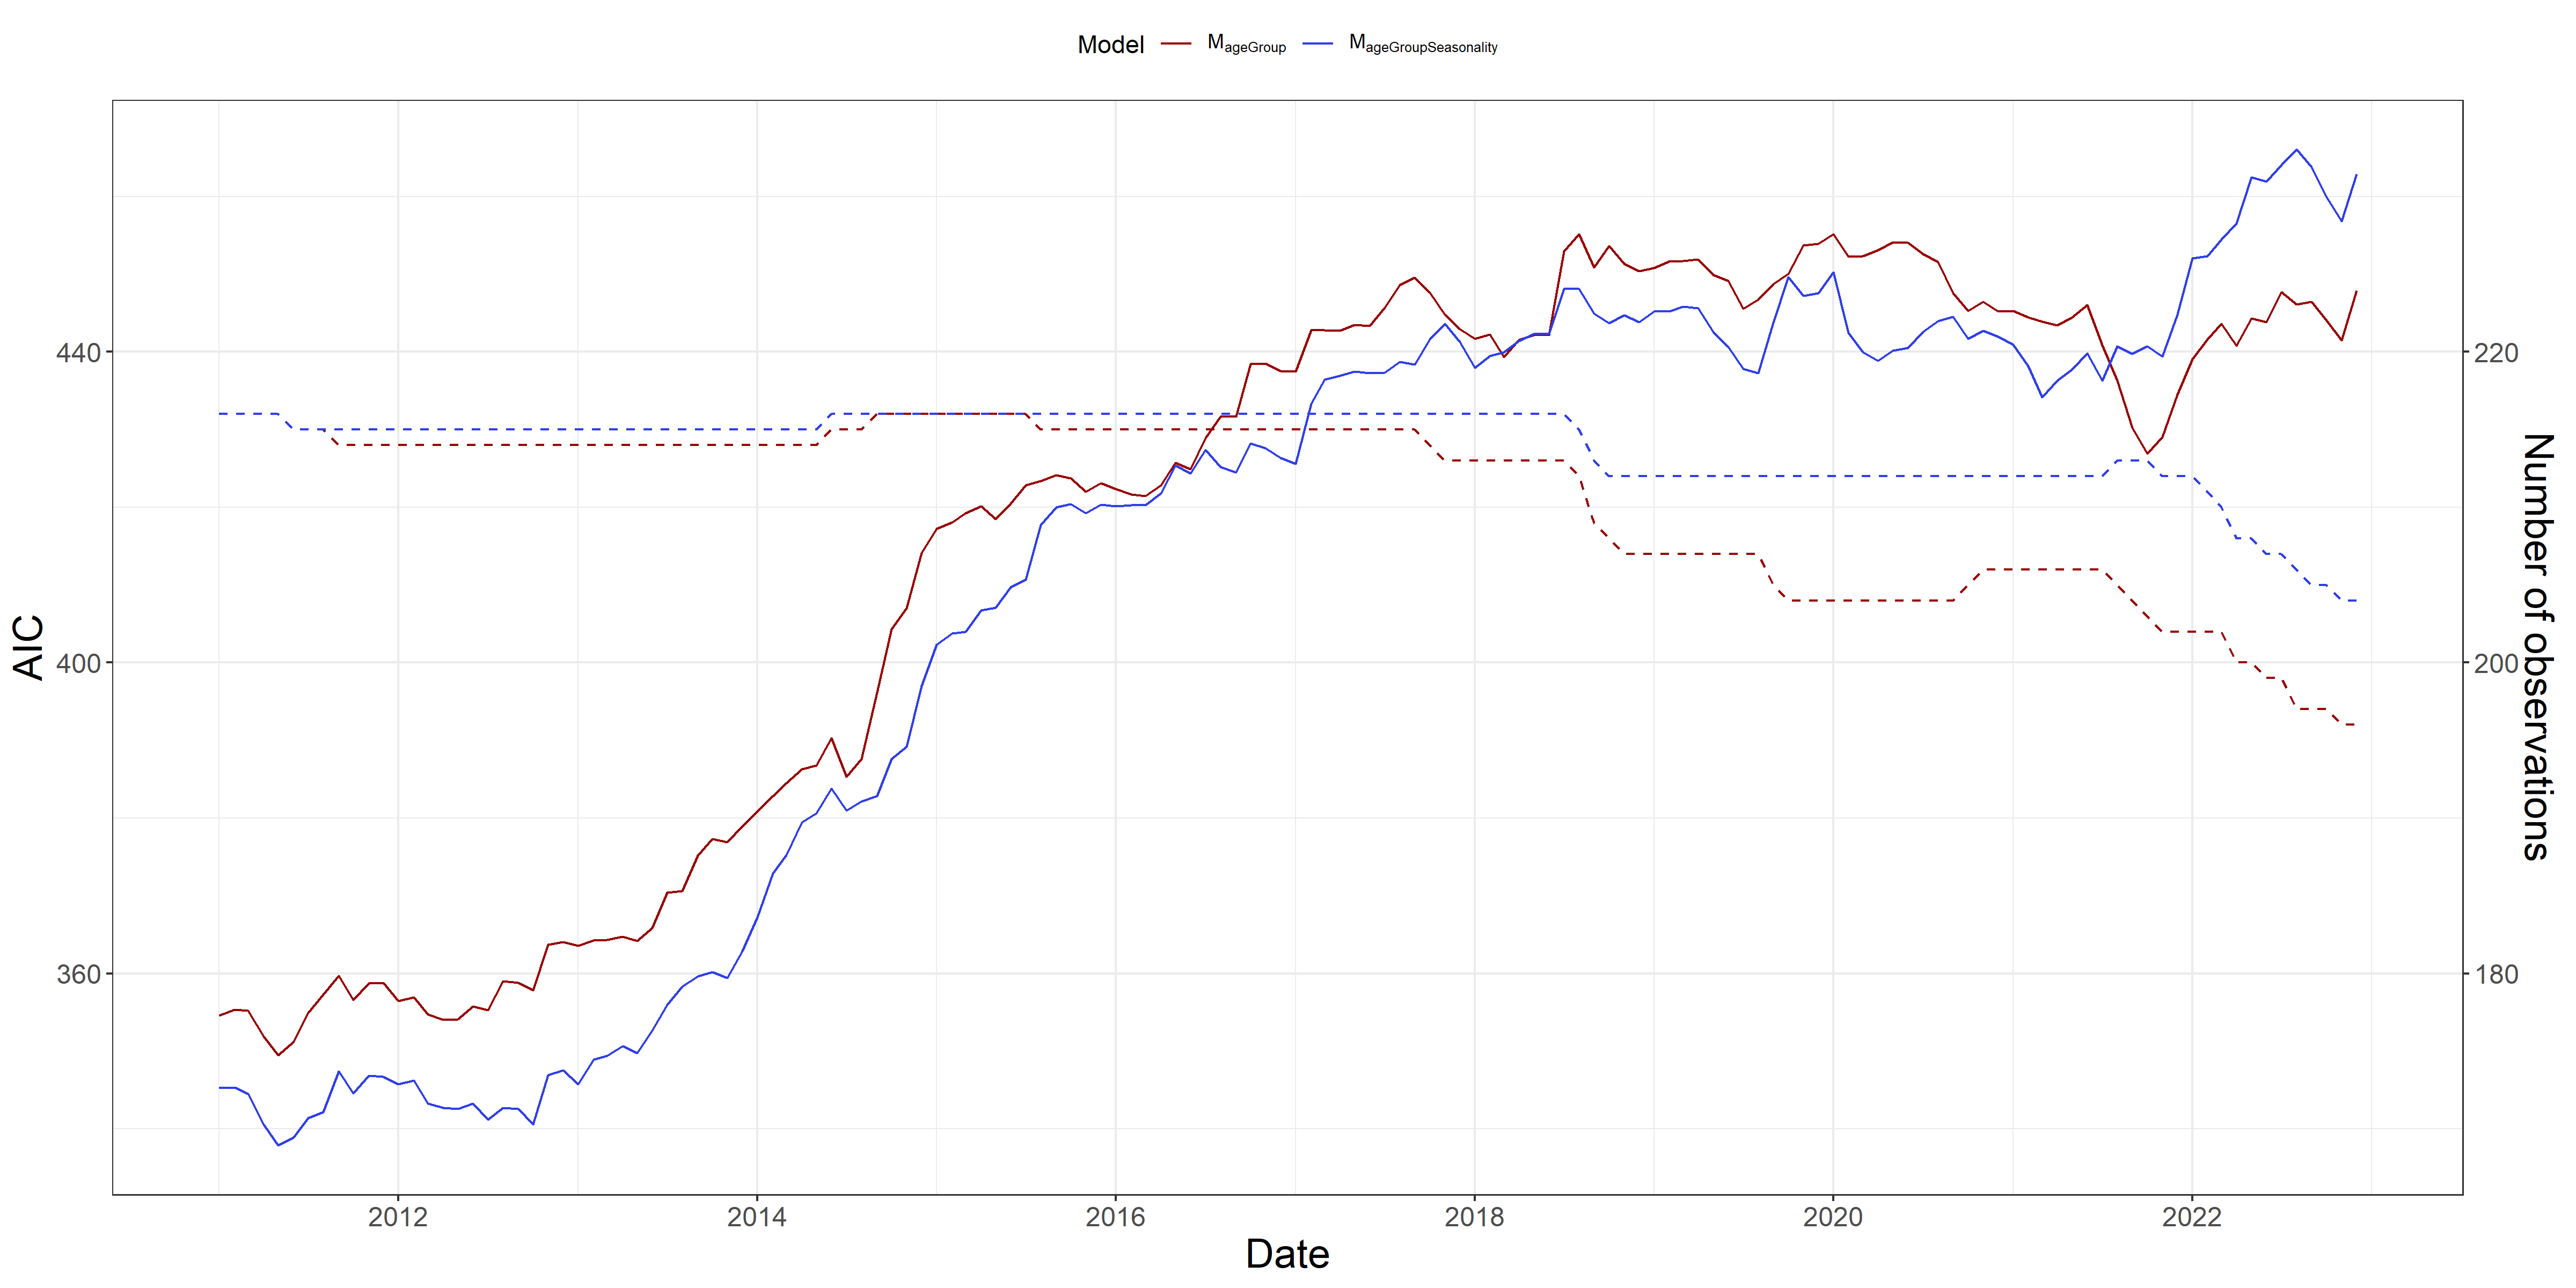
\includegraphics[width=1\linewidth]{../figures/AICxSTEC_PoisN}

\normalsize
\end{frame}

\begin{frame}{Agegroup parameters}
\protect\hypertarget{agegroup-parameters}{}
\tiny

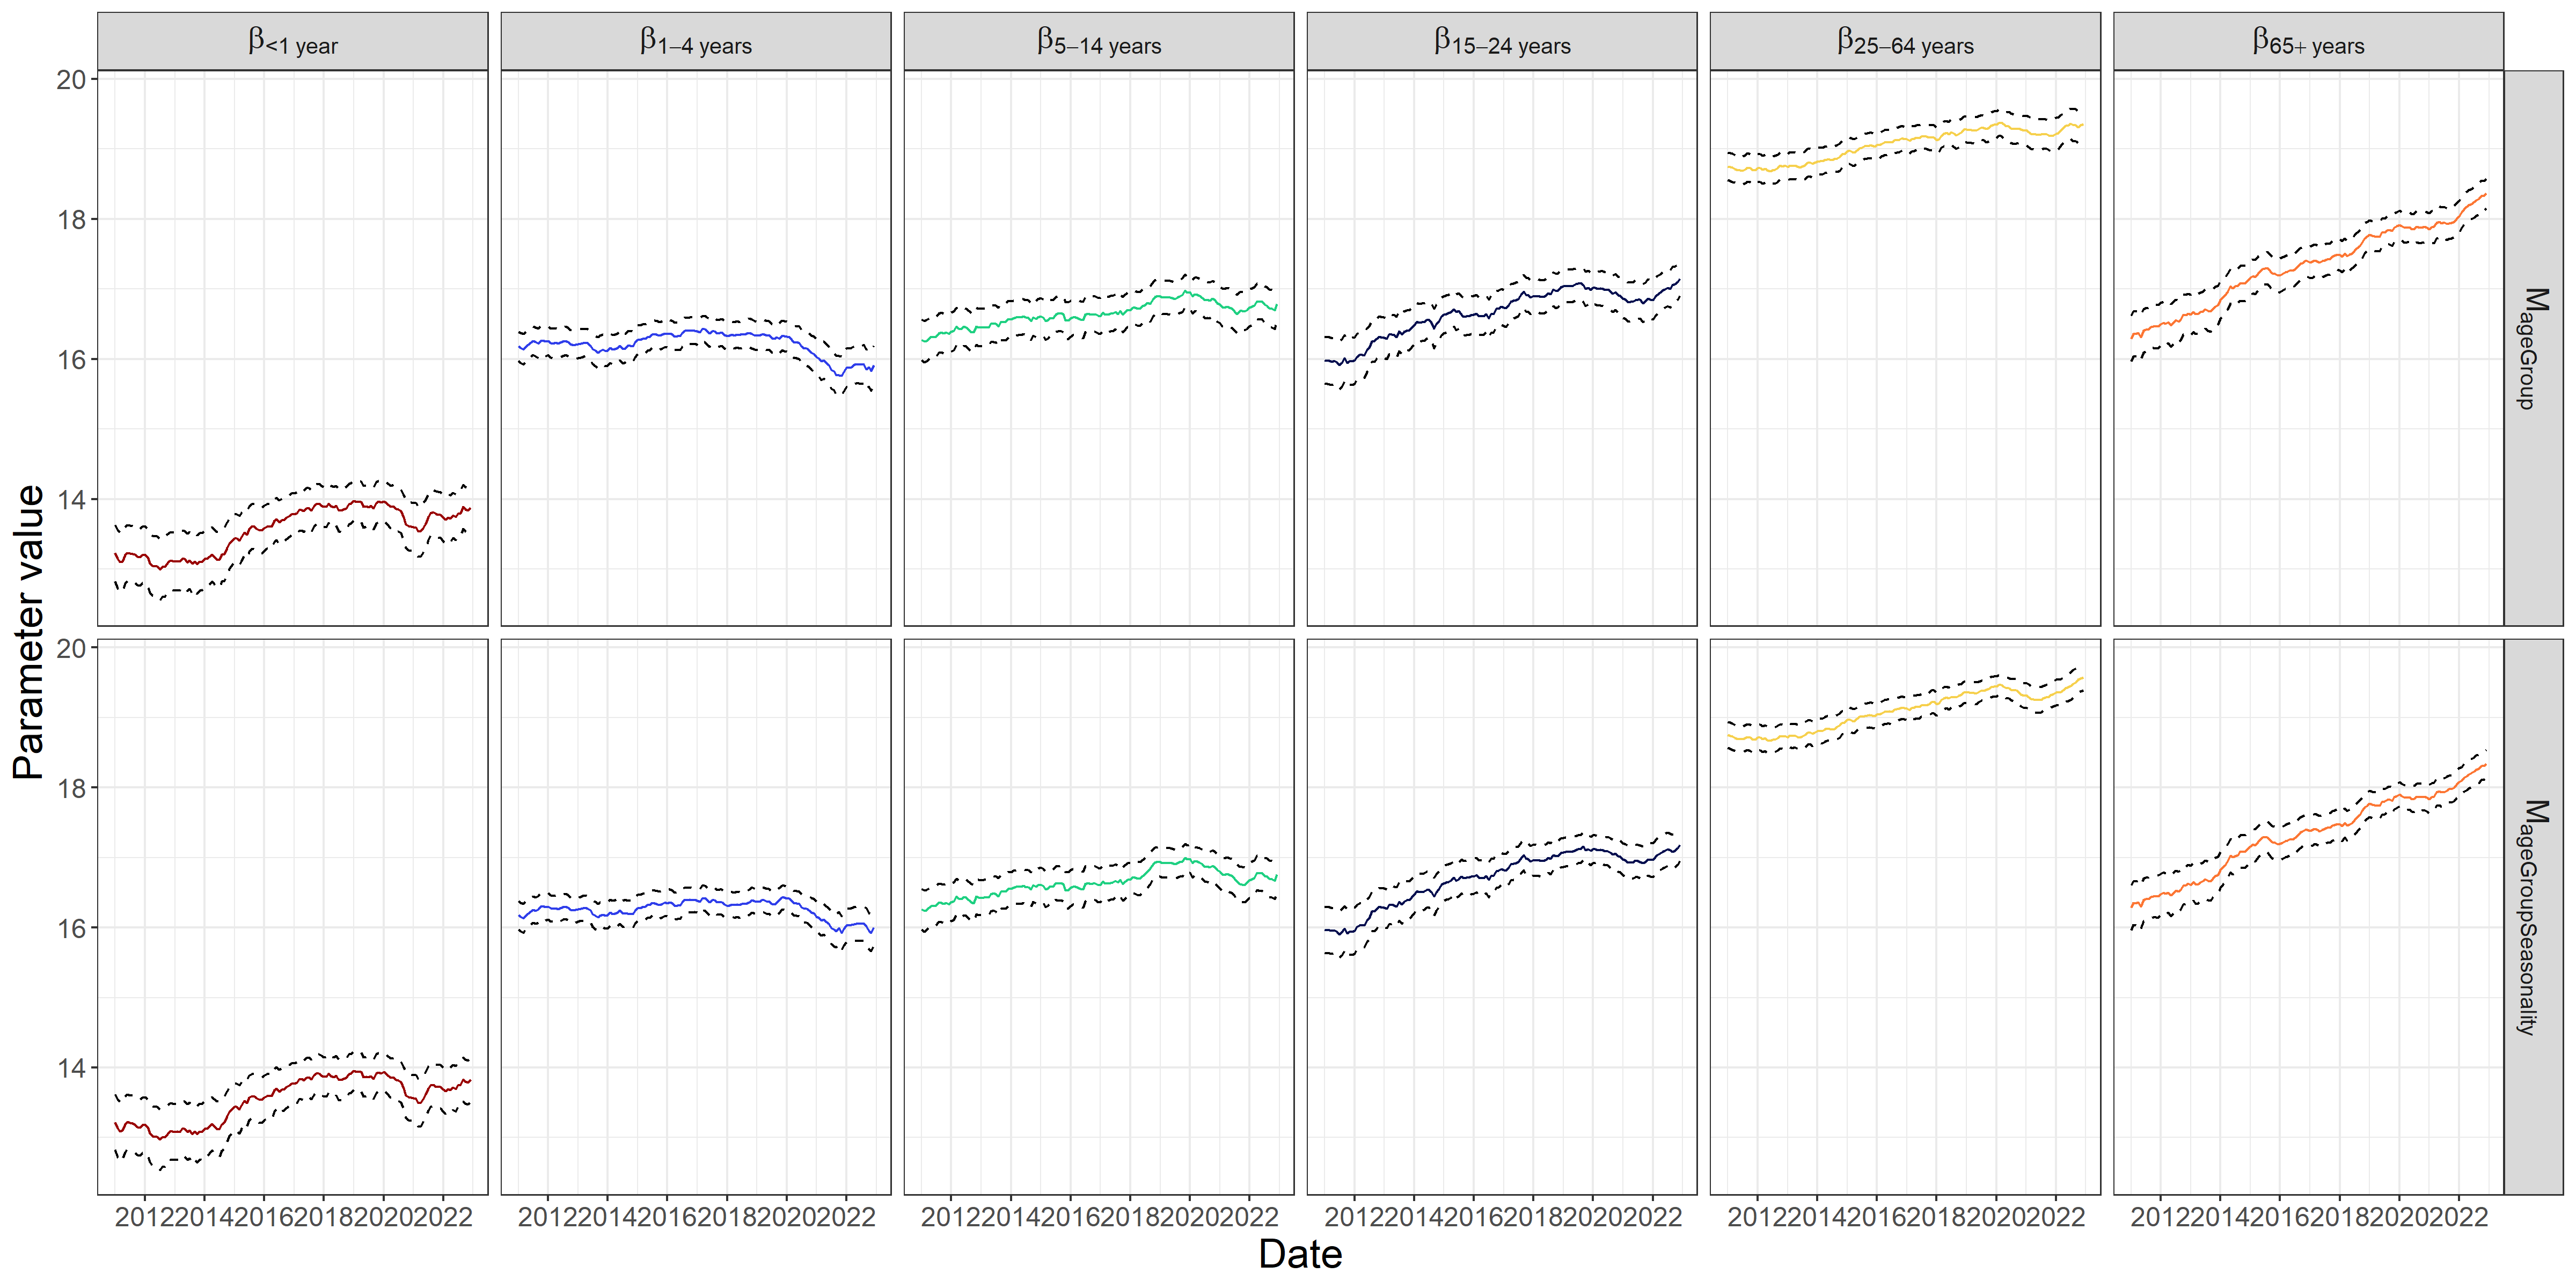
\includegraphics[width=1\linewidth]{../figures/ageGroupParxSTEC_PoisN}

\normalsize
\end{frame}

\begin{frame}{Seasonality parameters}
\protect\hypertarget{seasonality-parameters}{}
\tiny

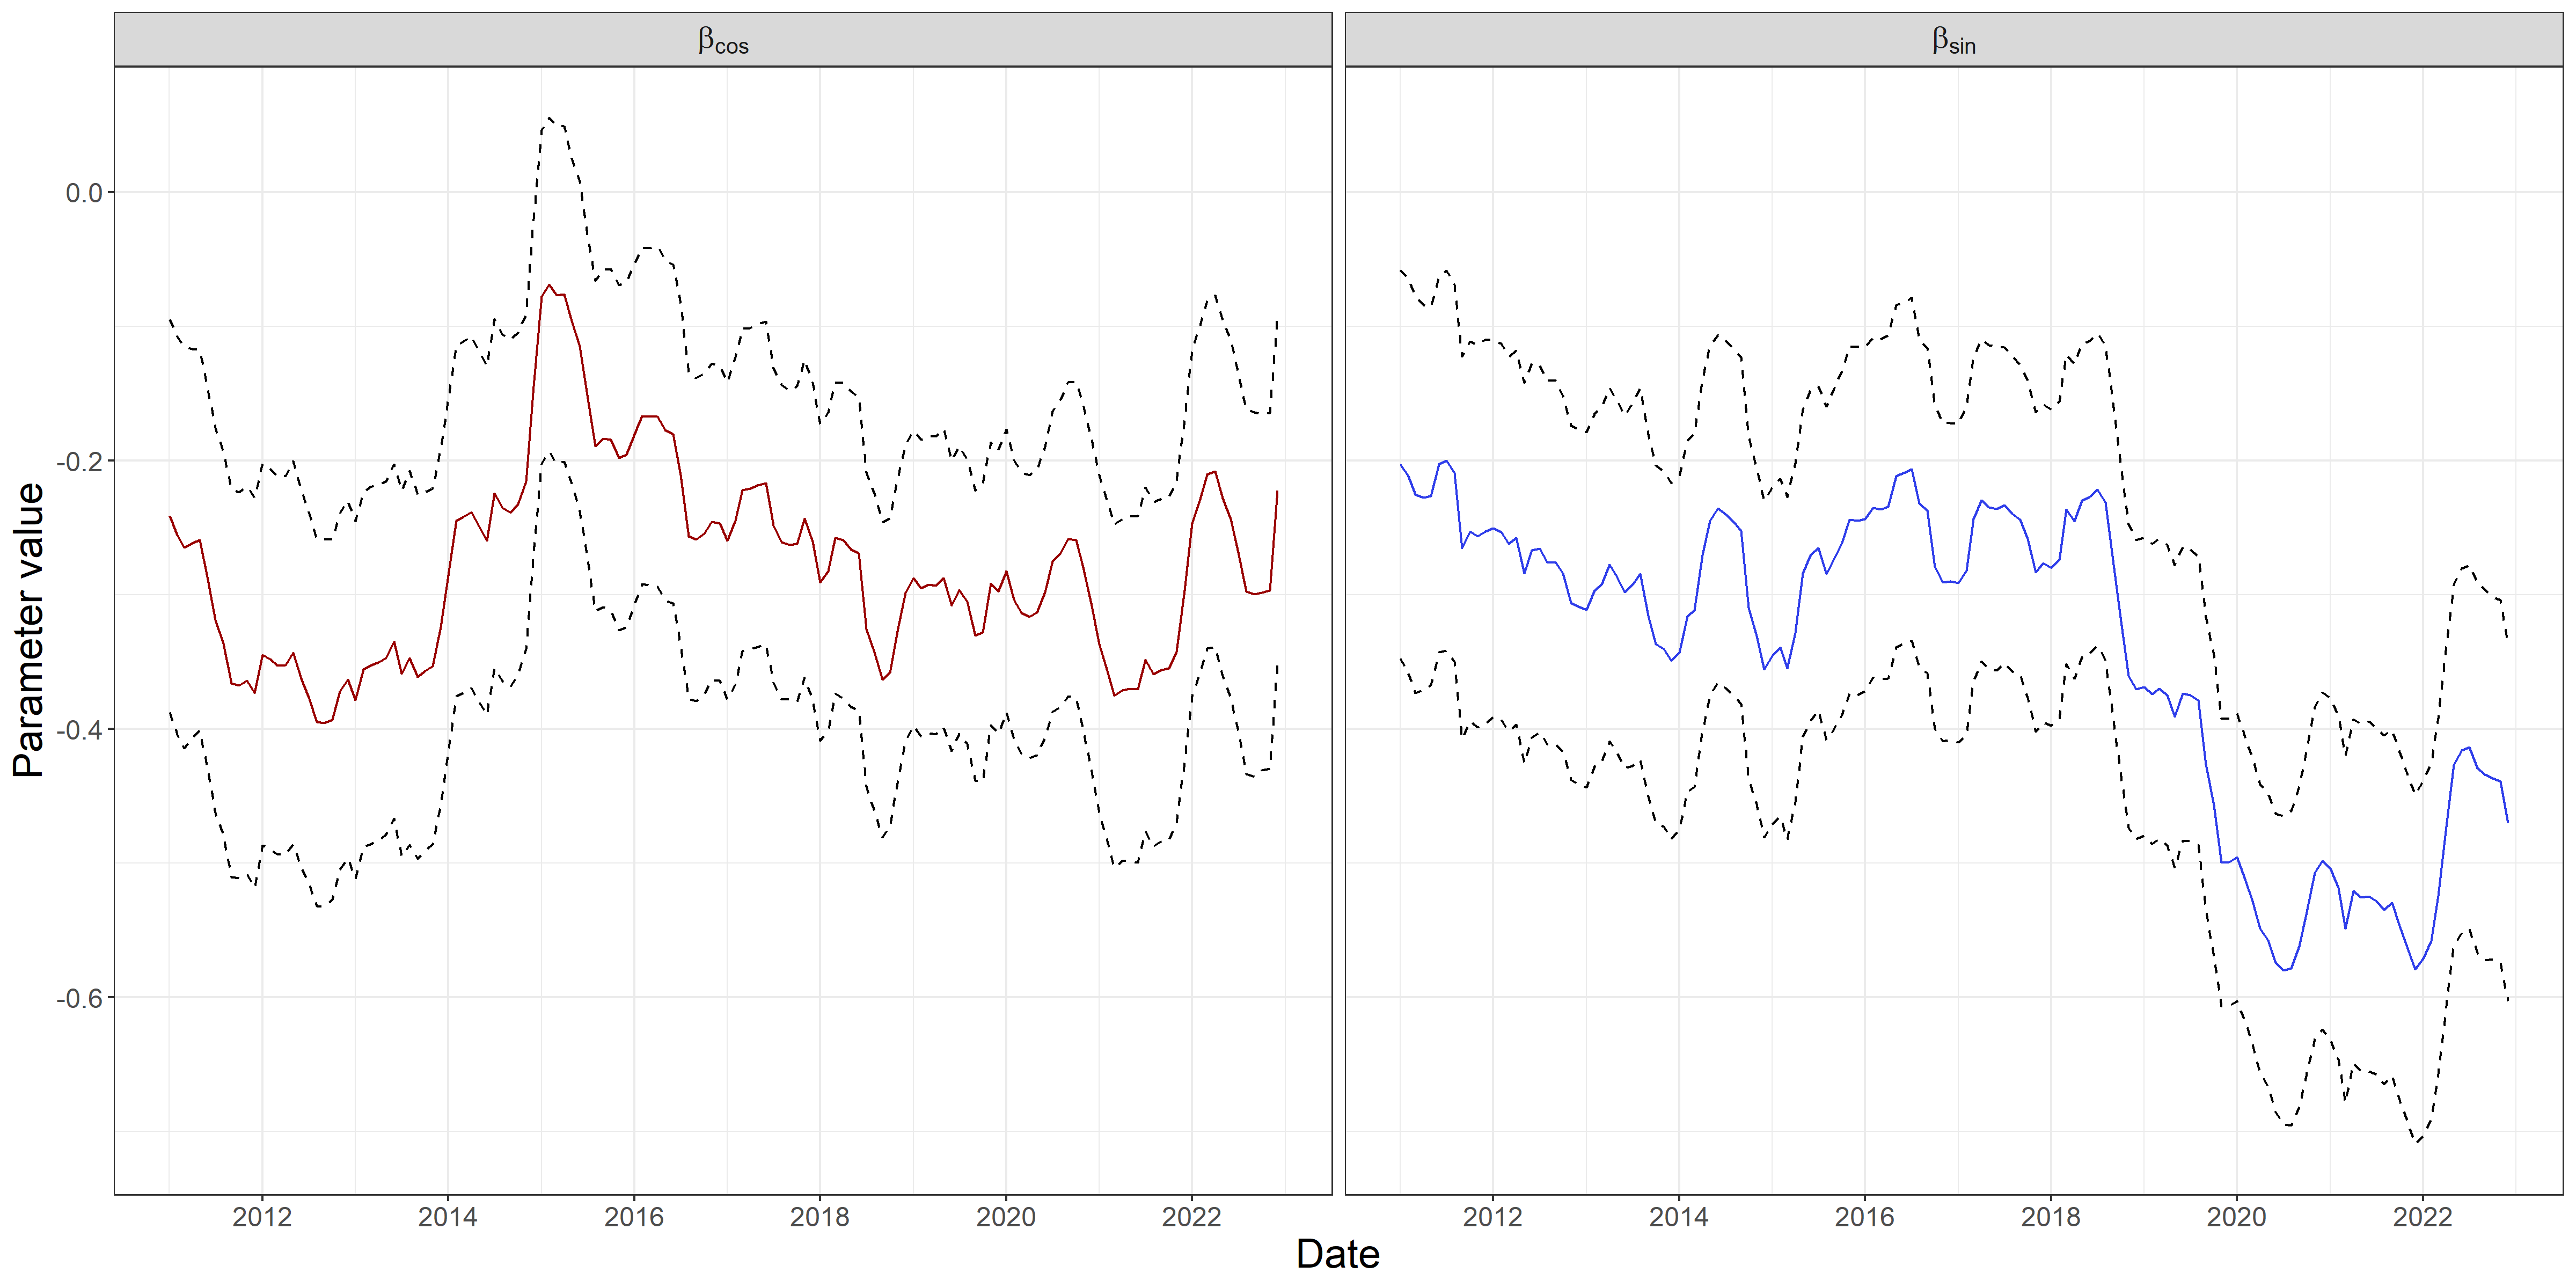
\includegraphics[width=1\linewidth]{../figures/SeasonalityParxSTEC_PoisN}

\normalsize
\end{frame}

\begin{frame}{Variance parameter}
\protect\hypertarget{variance-parameter}{}
\tiny

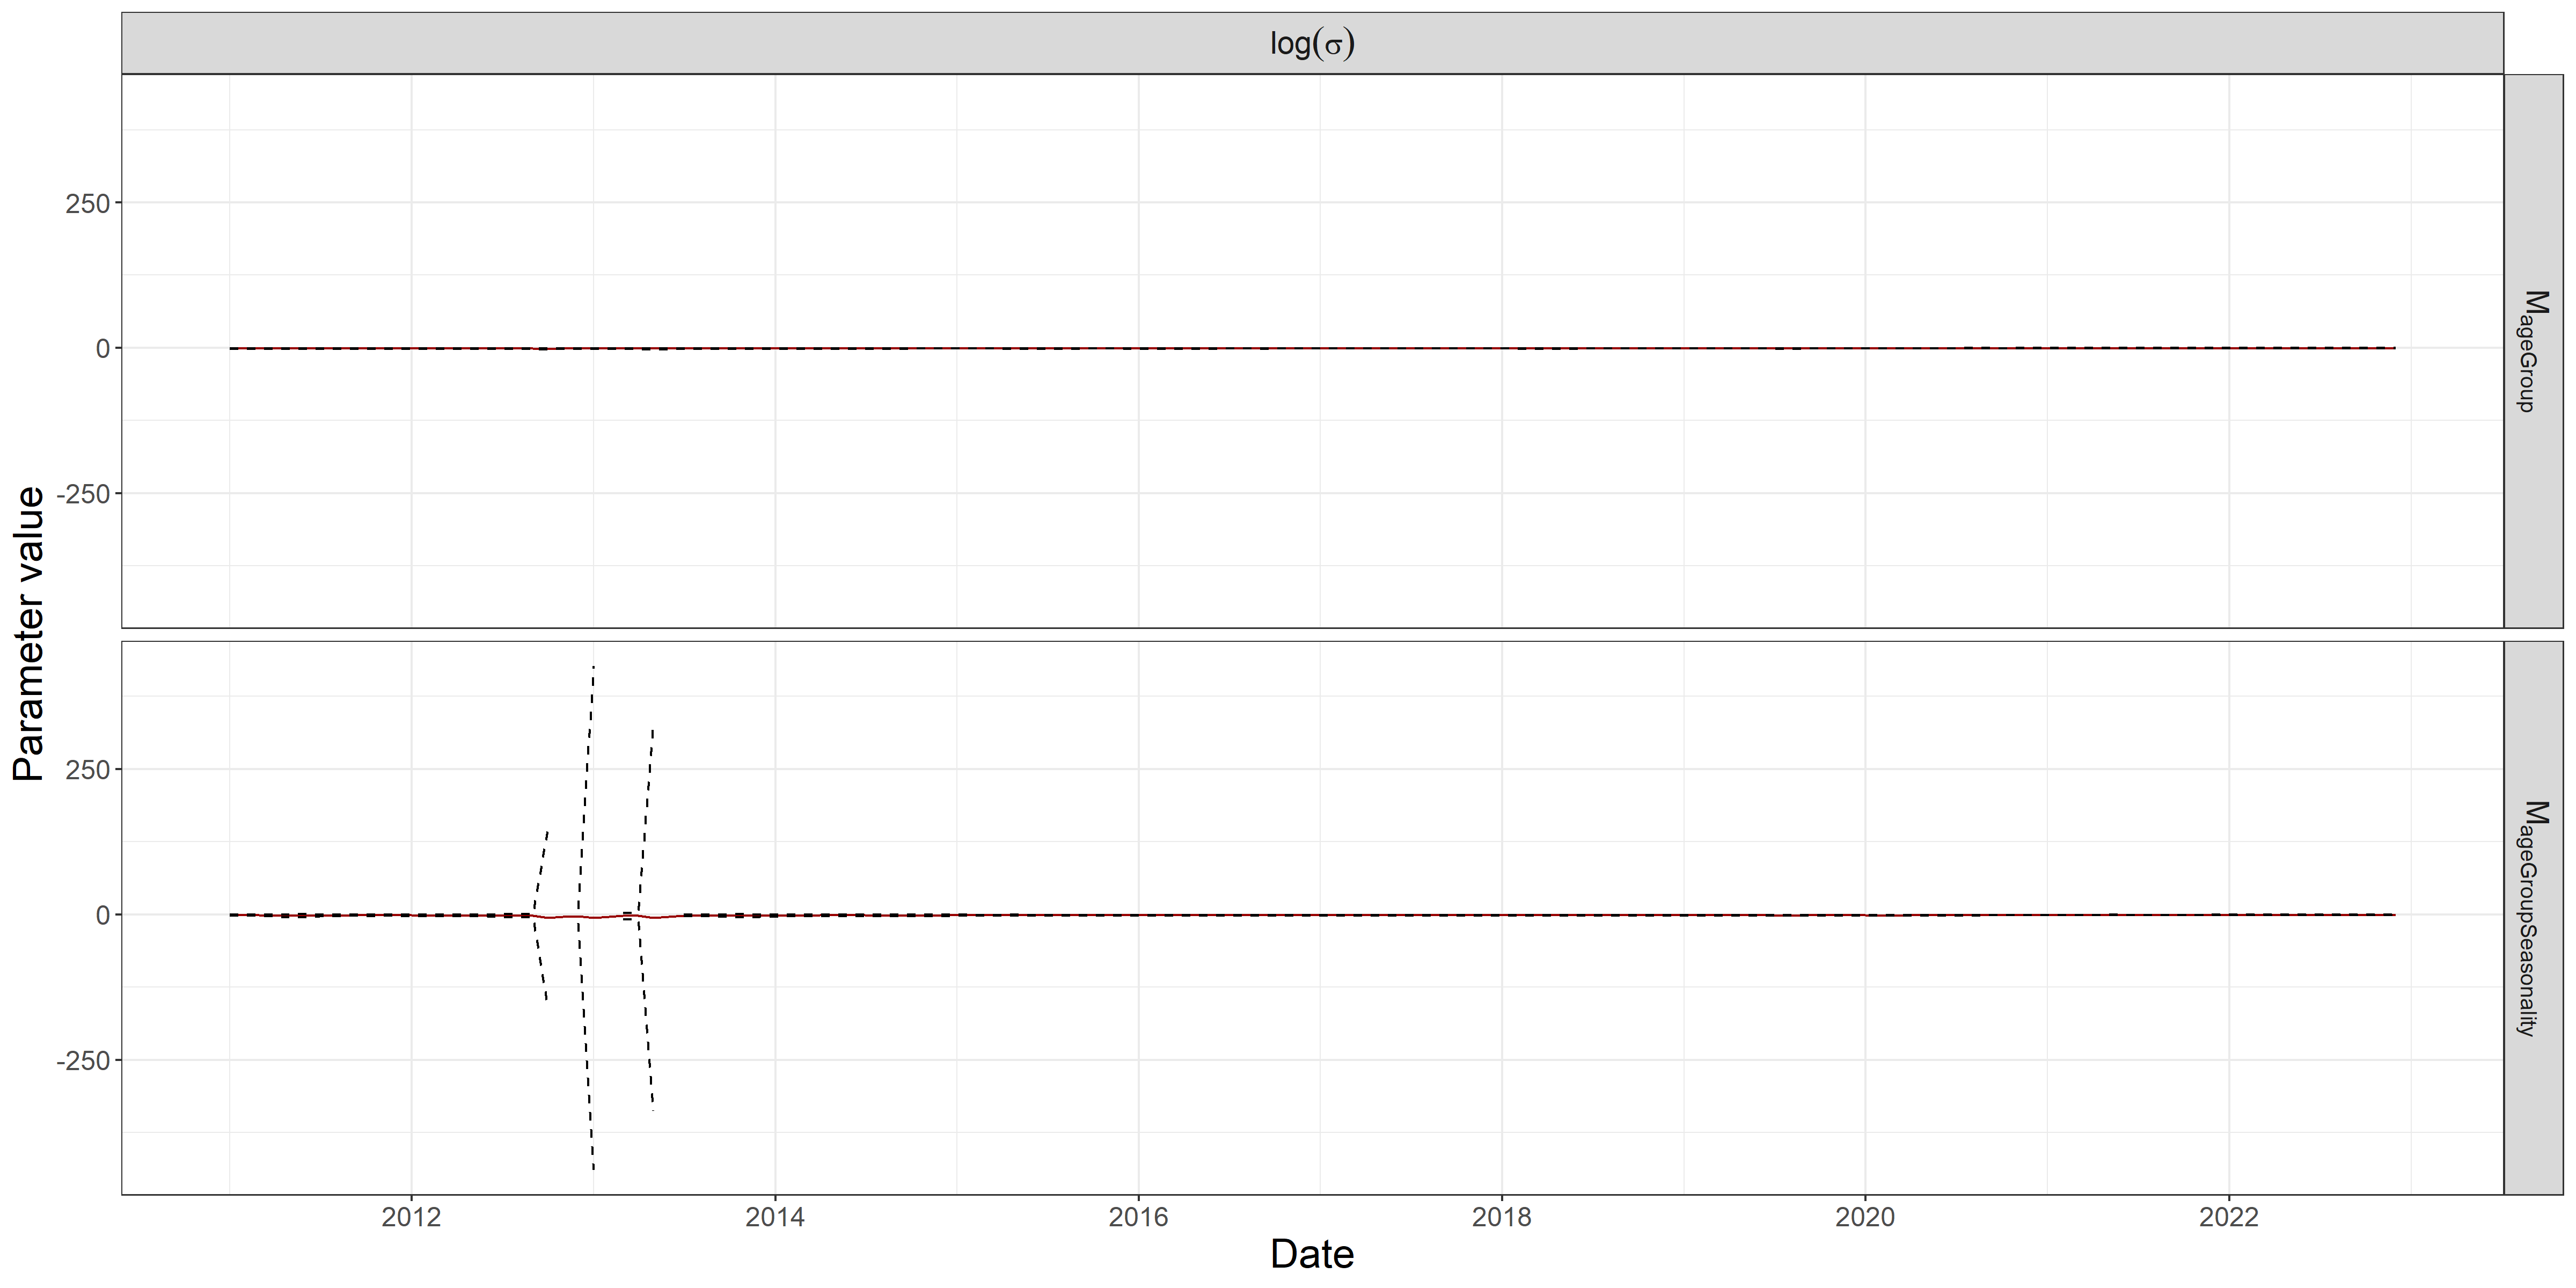
\includegraphics[width=1\linewidth]{../figures/log_sigmaxSTEC_PoisN}

\normalsize
\end{frame}

\begin{frame}{Outbreak detection}
\protect\hypertarget{outbreak-detection}{}
\tiny

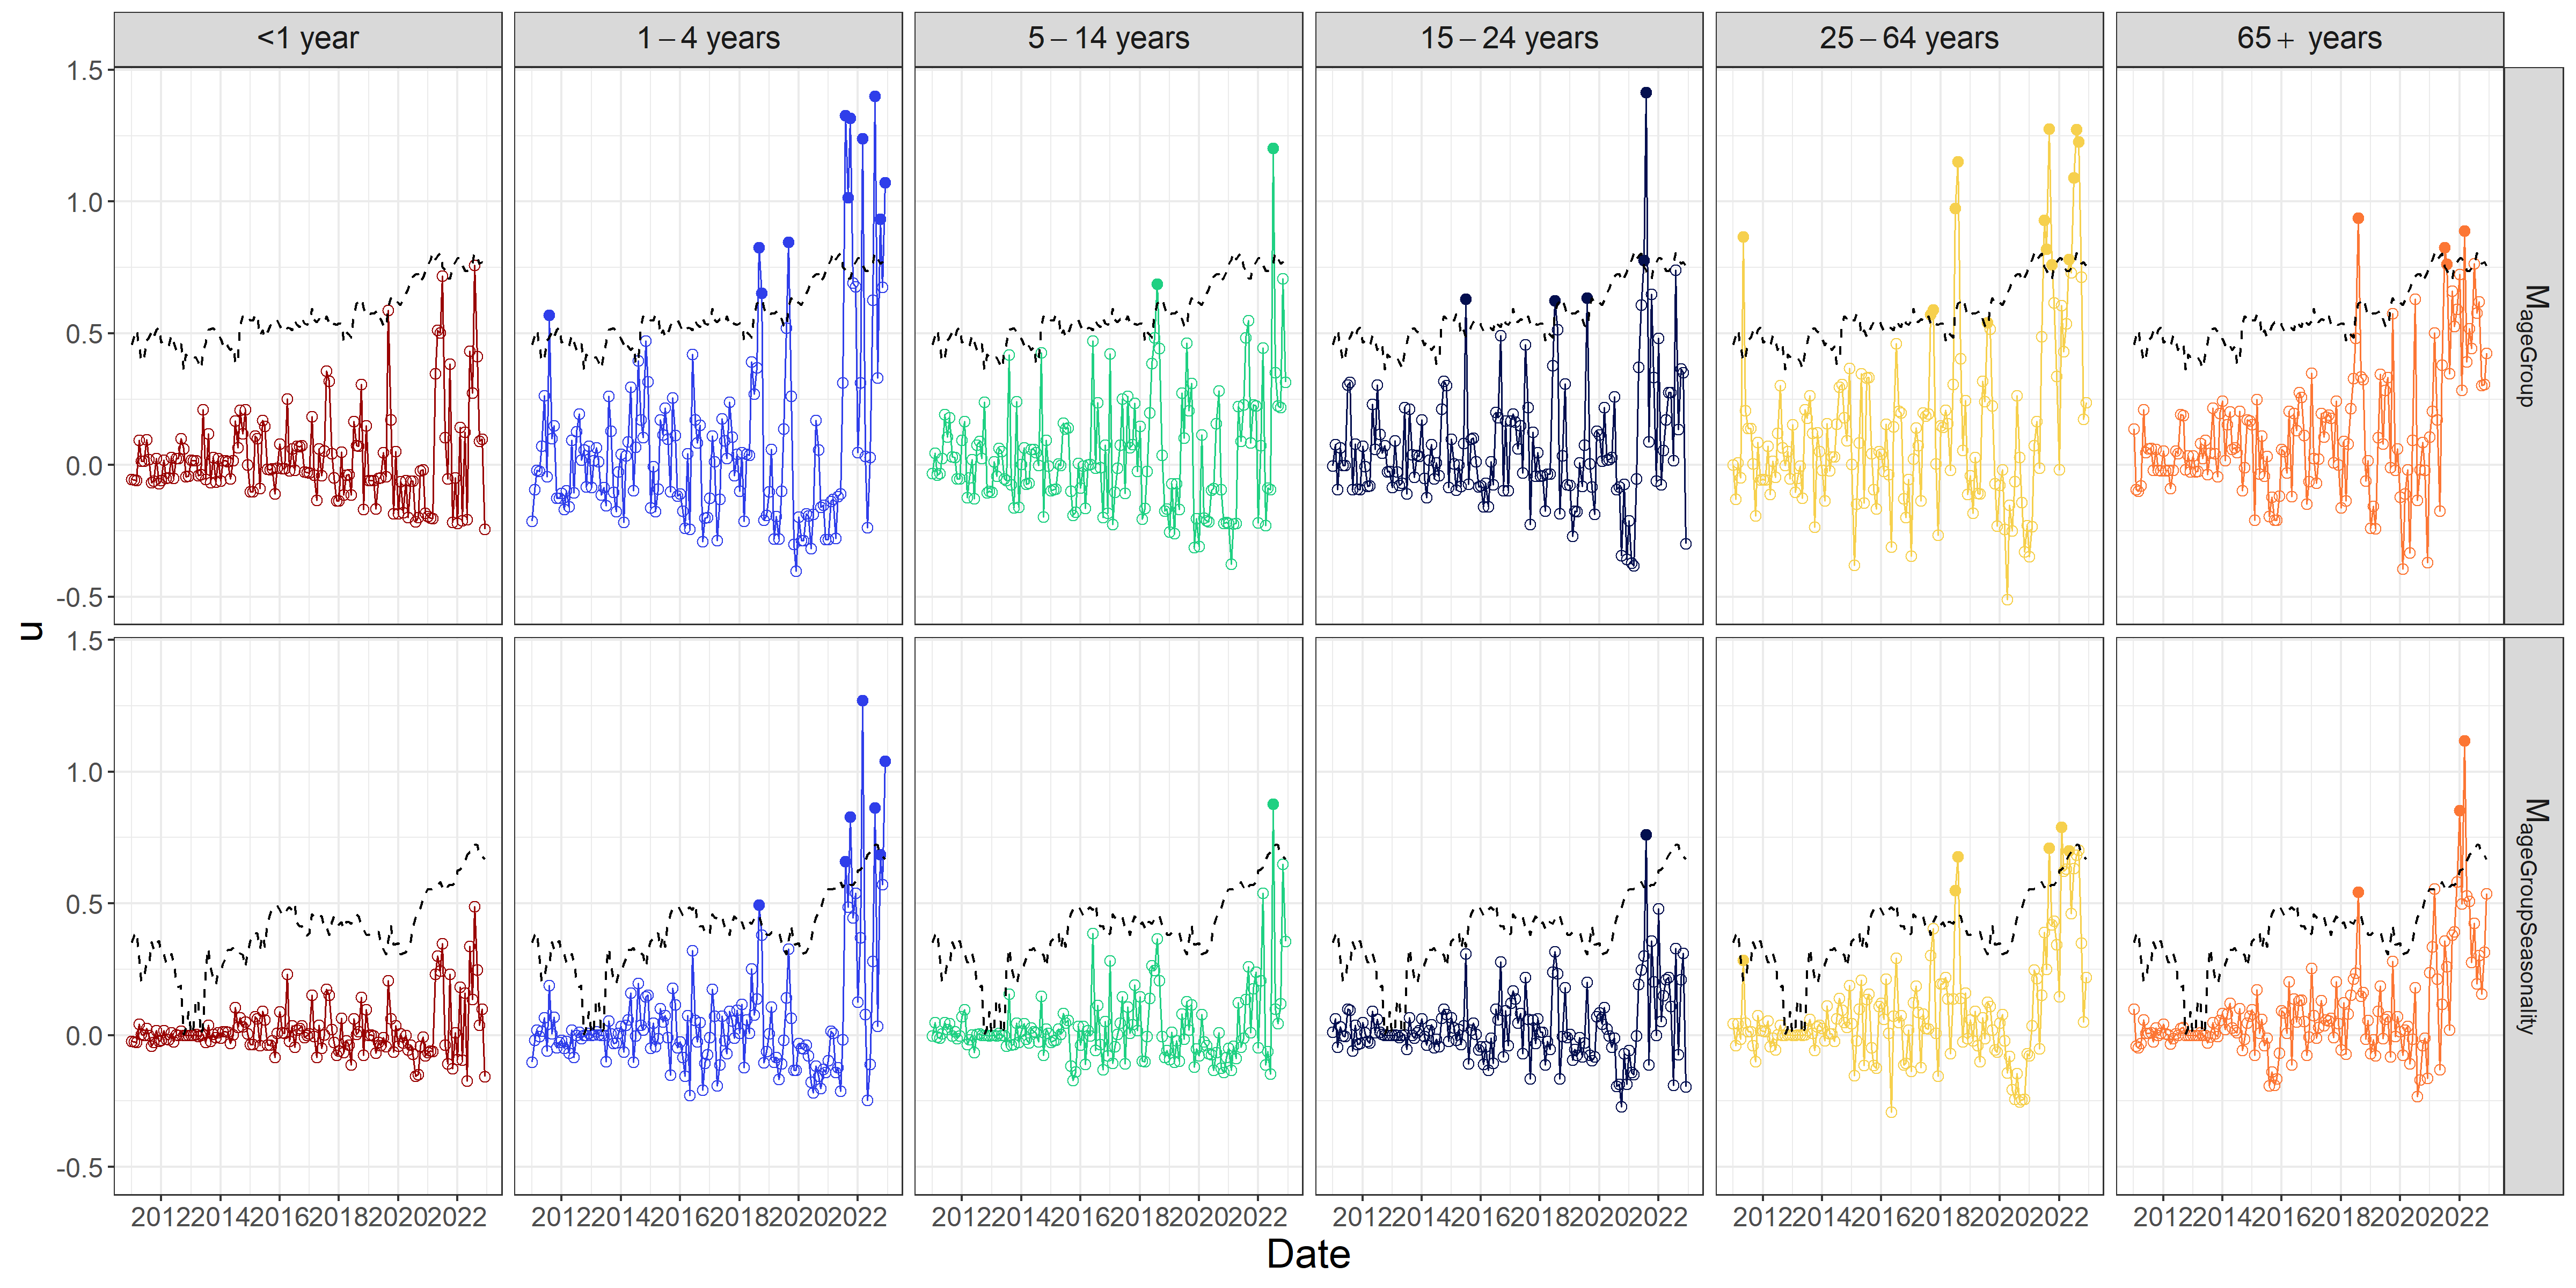
\includegraphics[width=1\linewidth]{../figures/OutbreakDetectionxSTEC_PoisN}

\normalsize
\end{frame}

\hypertarget{hierarchical-poisson-gamma-model}{%
\section{Hierarchical Poisson Gamma
model}\label{hierarchical-poisson-gamma-model}}

\begin{frame}{Hierarchical Poisson Gamma model}
\begin{subequations} \label{eq:PoisGam}
  \begin{alignat}{2}
    \boldsymbol{Y|u} &\sim \Pois (\boldsymbol{\lambda u}) \label{eq:pois_g0} \\ 
    \boldsymbol{u} &\sim \G(\boldsymbol 1/\phi,\phi) \label{eq:pois_g1}
  \end{alignat}
\end{subequations}
\end{frame}

\hypertarget{implementation-1}{%
\subsection{Implementation}\label{implementation-1}}

\begin{frame}[fragile]{Implementation}
\tiny

\begin{Shaded}
\begin{Highlighting}[]
\PreprocessorTok{\#include }\ImportTok{\textless{}TMB.hpp\textgreater{}}\PreprocessorTok{              }\CommentTok{// Links in the TMB libraries}

\KeywordTok{template}\OperatorTok{\textless{}}\KeywordTok{class}\NormalTok{ Type}\OperatorTok{\textgreater{}}
\NormalTok{Type objective\_function}\OperatorTok{\textless{}}\NormalTok{Type}\OperatorTok{\textgreater{}::}\KeywordTok{operator}\OperatorTok{()} \OperatorTok{()}
\OperatorTok{\{}
\NormalTok{  DATA\_VECTOR}\OperatorTok{(}\NormalTok{y}\OperatorTok{);}                               \CommentTok{// Data vector transmitted from R}
\NormalTok{  DATA\_VECTOR}\OperatorTok{(}\NormalTok{x}\OperatorTok{);}                       \CommentTok{// Data vector transmitted from R}
\NormalTok{  DATA\_MATRIX}\OperatorTok{(}\NormalTok{X}\OperatorTok{);}                       \CommentTok{// Design matrix transmitted from R}
  
  \CommentTok{// Parameters}
\NormalTok{  PARAMETER\_VECTOR}\OperatorTok{(}\NormalTok{beta}\OperatorTok{);}         \CommentTok{// Parameter value transmitted from R}
\NormalTok{  PARAMETER}\OperatorTok{(}\NormalTok{log\_phi\_u}\OperatorTok{);}             \CommentTok{// Parameter value transmitted from R}
  
\NormalTok{  vector}\OperatorTok{\textless{}}\NormalTok{Type}\OperatorTok{\textgreater{}}\NormalTok{ lambda  }\OperatorTok{=}\NormalTok{ exp}\OperatorTok{(}\NormalTok{X}\OperatorTok{*}\NormalTok{beta}\OperatorTok{{-}}\NormalTok{log}\OperatorTok{(}\NormalTok{x}\OperatorTok{));} \CommentTok{// Construct the model parameters}
\NormalTok{  Type phi\_u }\OperatorTok{=}\NormalTok{ exp}\OperatorTok{(}\NormalTok{log\_phi\_u}\OperatorTok{);} \CommentTok{// ... and the model parameters}
  
\NormalTok{  Type r }\OperatorTok{=} \DecValTok{1}\OperatorTok{/}\NormalTok{phi\_u}\OperatorTok{;} \CommentTok{// Construct the size}
\NormalTok{  vector}\OperatorTok{\textless{}}\NormalTok{Type}\OperatorTok{\textgreater{}}\NormalTok{ p }\OperatorTok{=} \DecValTok{1}\OperatorTok{/(}\NormalTok{lambda}\OperatorTok{*}\NormalTok{phi\_u}\OperatorTok{+}\DecValTok{1}\OperatorTok{);} \CommentTok{// ... and the probability parameter}
  
\NormalTok{  Type f }\OperatorTok{=} \OperatorTok{{-}}\NormalTok{sum}\OperatorTok{(}\NormalTok{dnbinom}\OperatorTok{(}\NormalTok{y}\OperatorTok{,}\NormalTok{ r}\OperatorTok{,}\NormalTok{ p}\OperatorTok{,}\KeywordTok{true}\OperatorTok{));} \CommentTok{// Calculate the "objective function"}
  
  \ControlFlowTok{return}\NormalTok{ f}\OperatorTok{;}
\OperatorTok{\}}
\end{Highlighting}
\end{Shaded}

\normalsize
\end{frame}

\hypertarget{results-1}{%
\subsection{Results}\label{results-1}}

\begin{frame}{Model performance}
\protect\hypertarget{model-performance-1}{}
\tiny

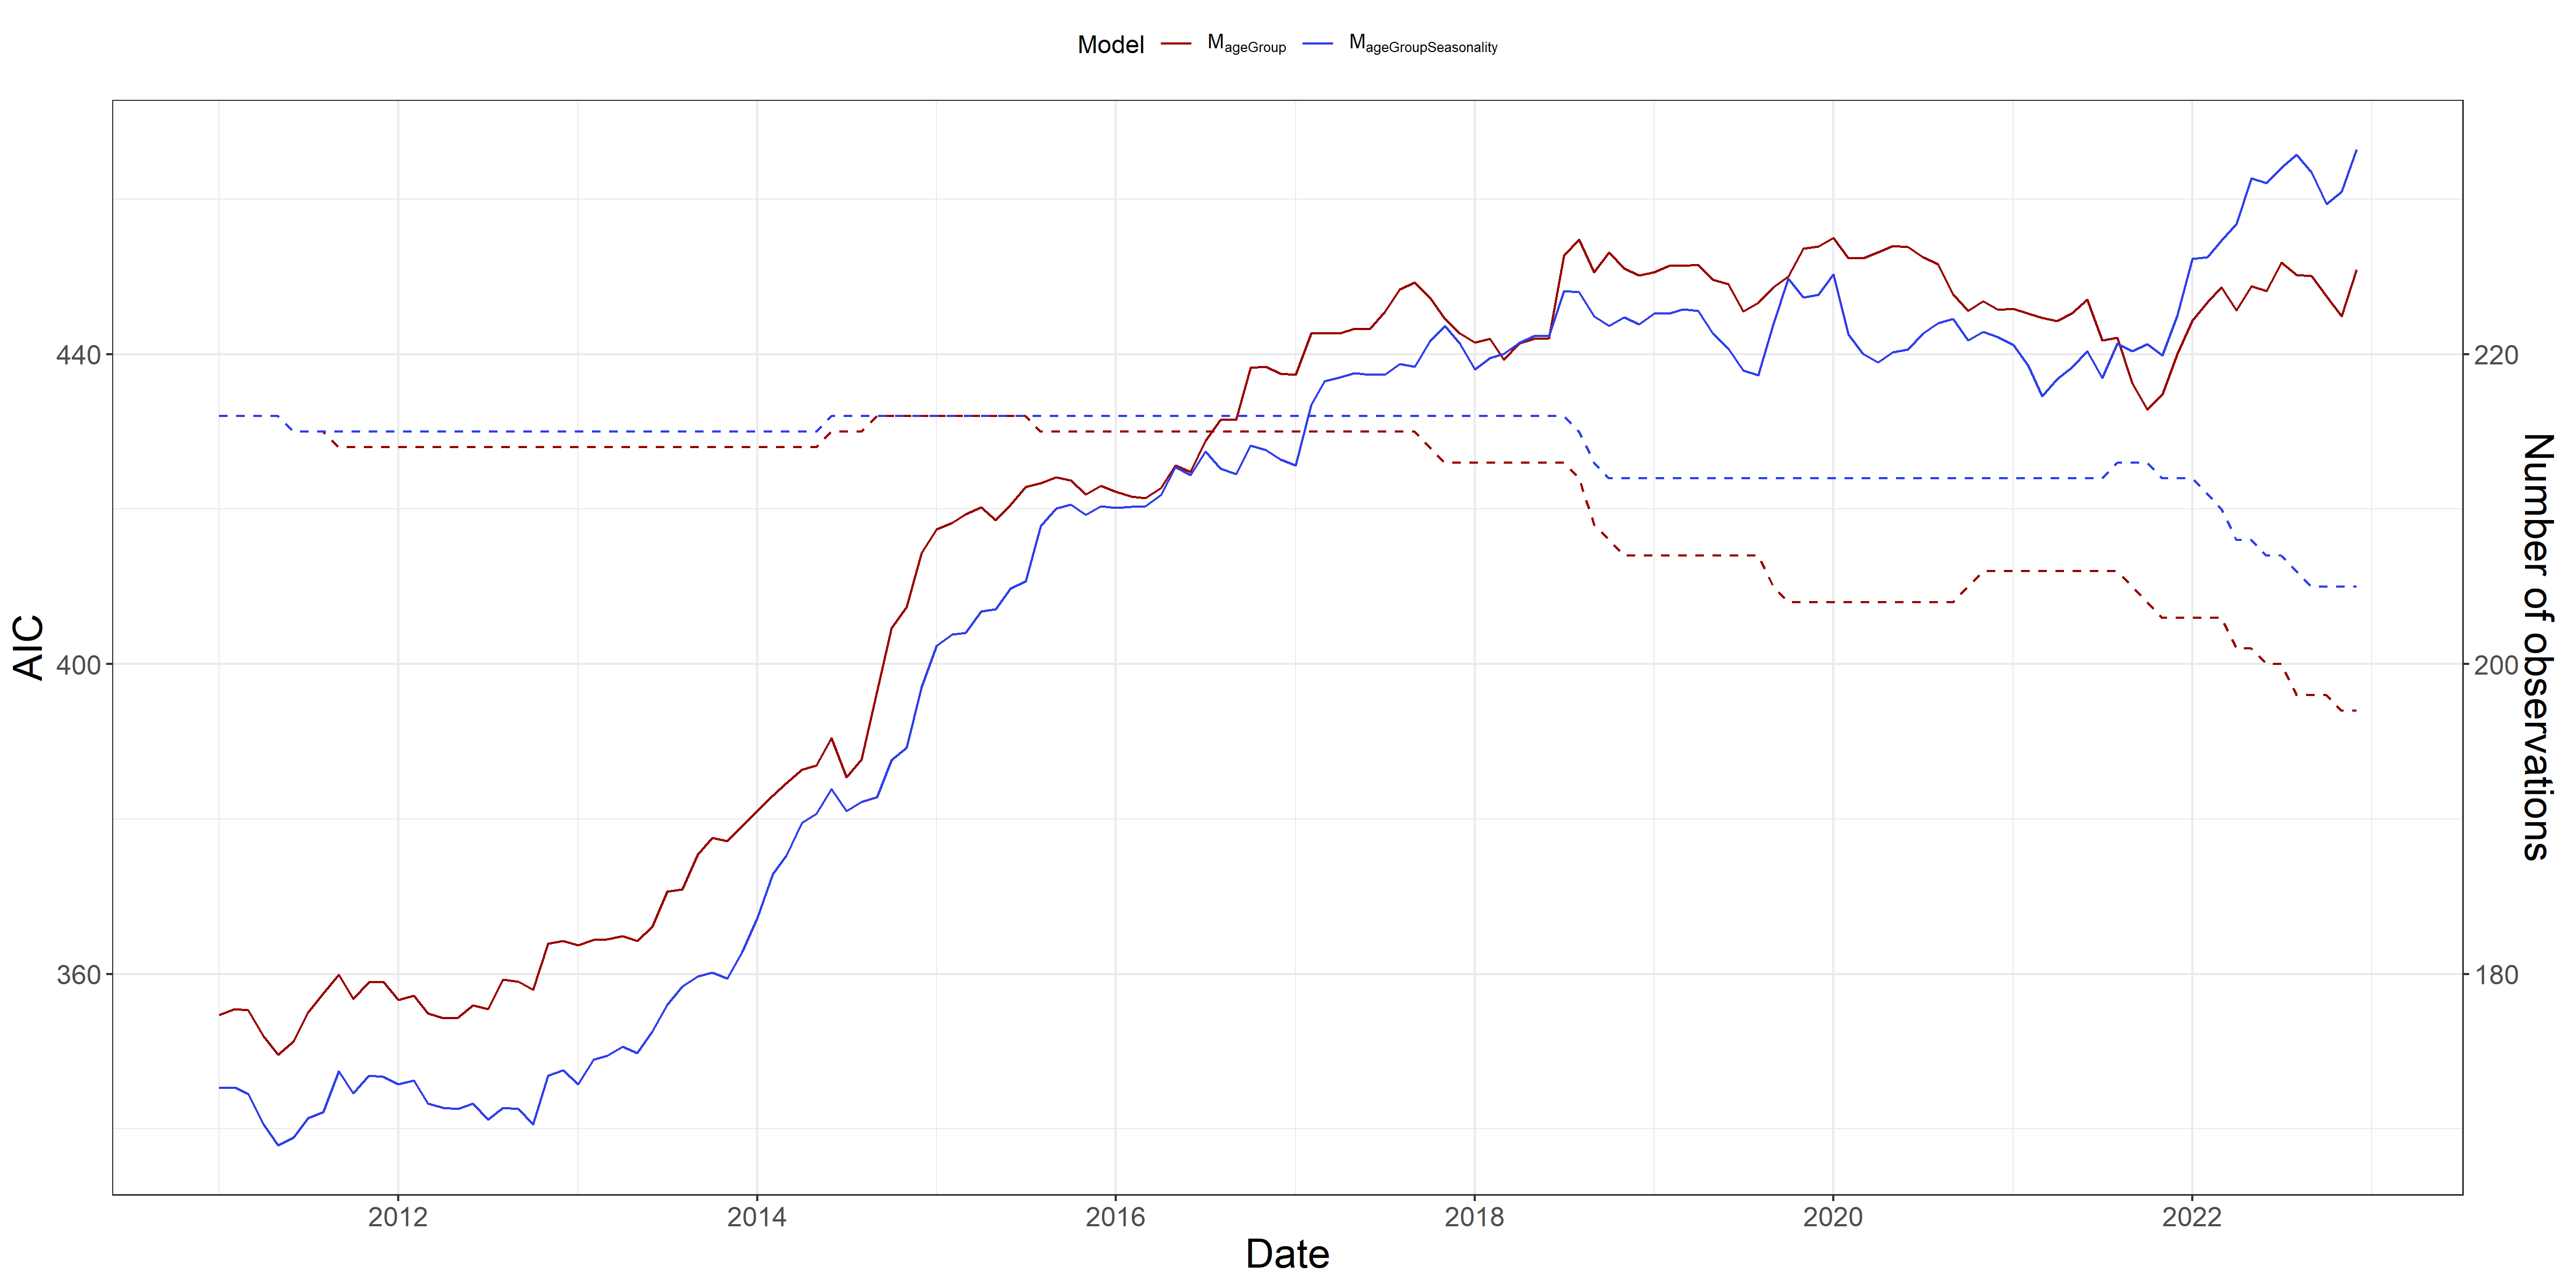
\includegraphics[width=1\linewidth]{../figures/AICxSTEC_PoisG}

\normalsize
\end{frame}

\begin{frame}{Agegroup parameters}
\protect\hypertarget{agegroup-parameters-1}{}
\tiny

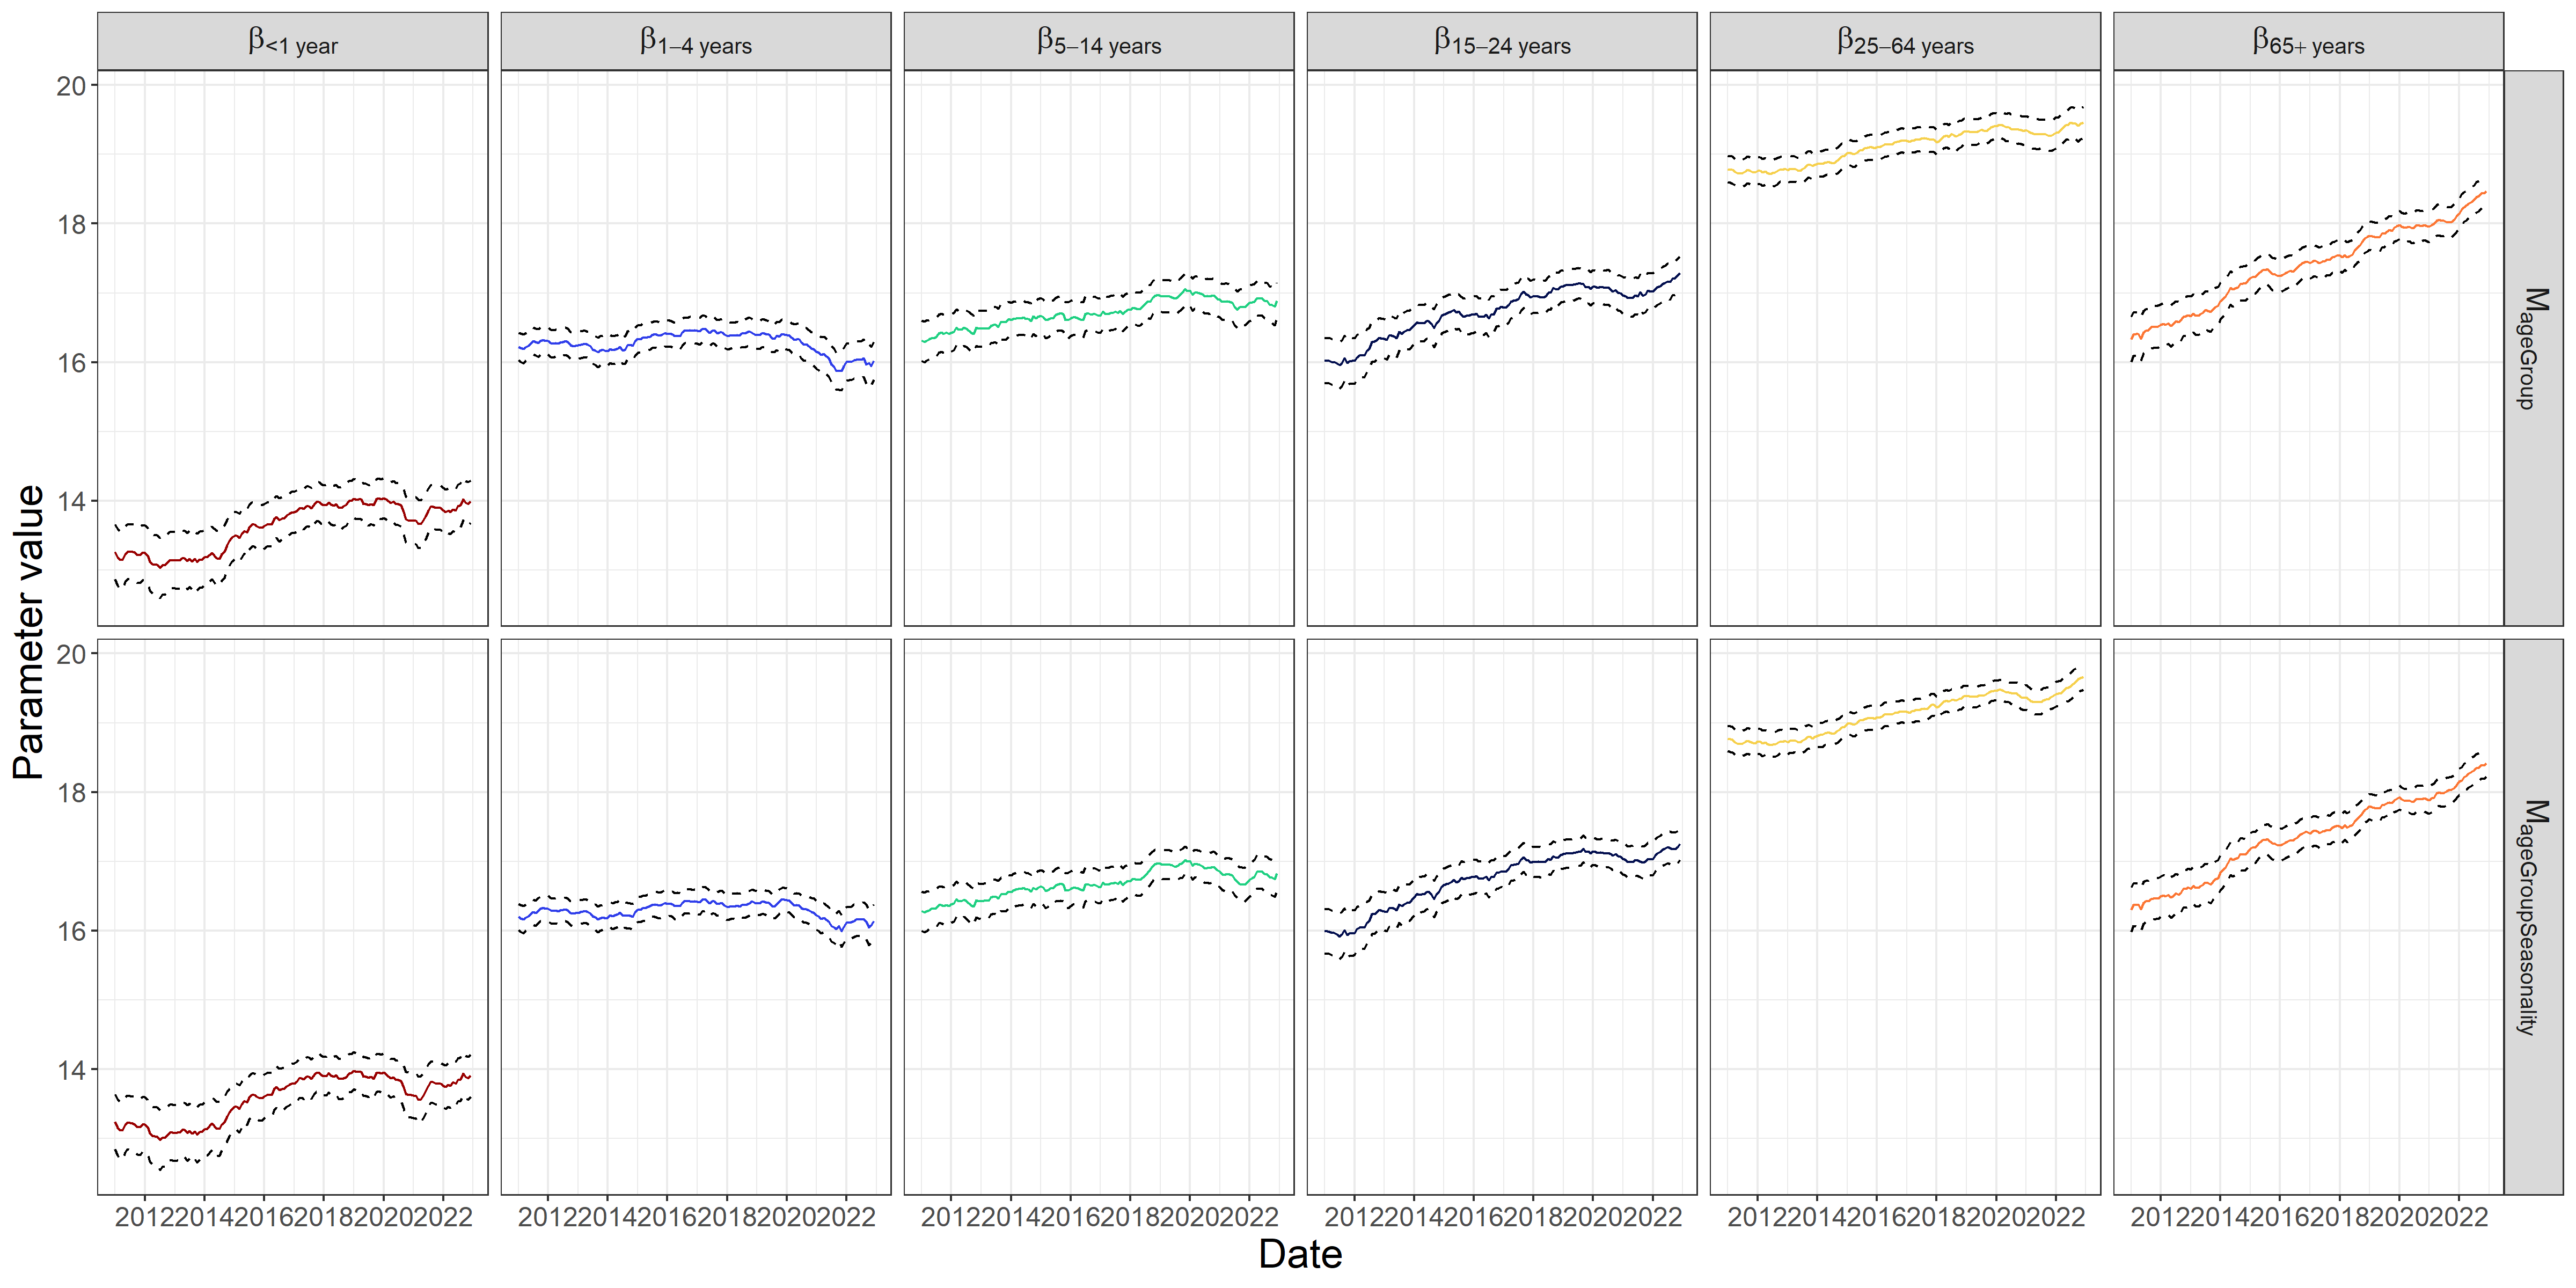
\includegraphics[width=1\linewidth]{../figures/ageGroupParxSTEC_PoisG}

\normalsize
\end{frame}

\begin{frame}{Seasonality parameters}
\protect\hypertarget{seasonality-parameters-1}{}
\tiny

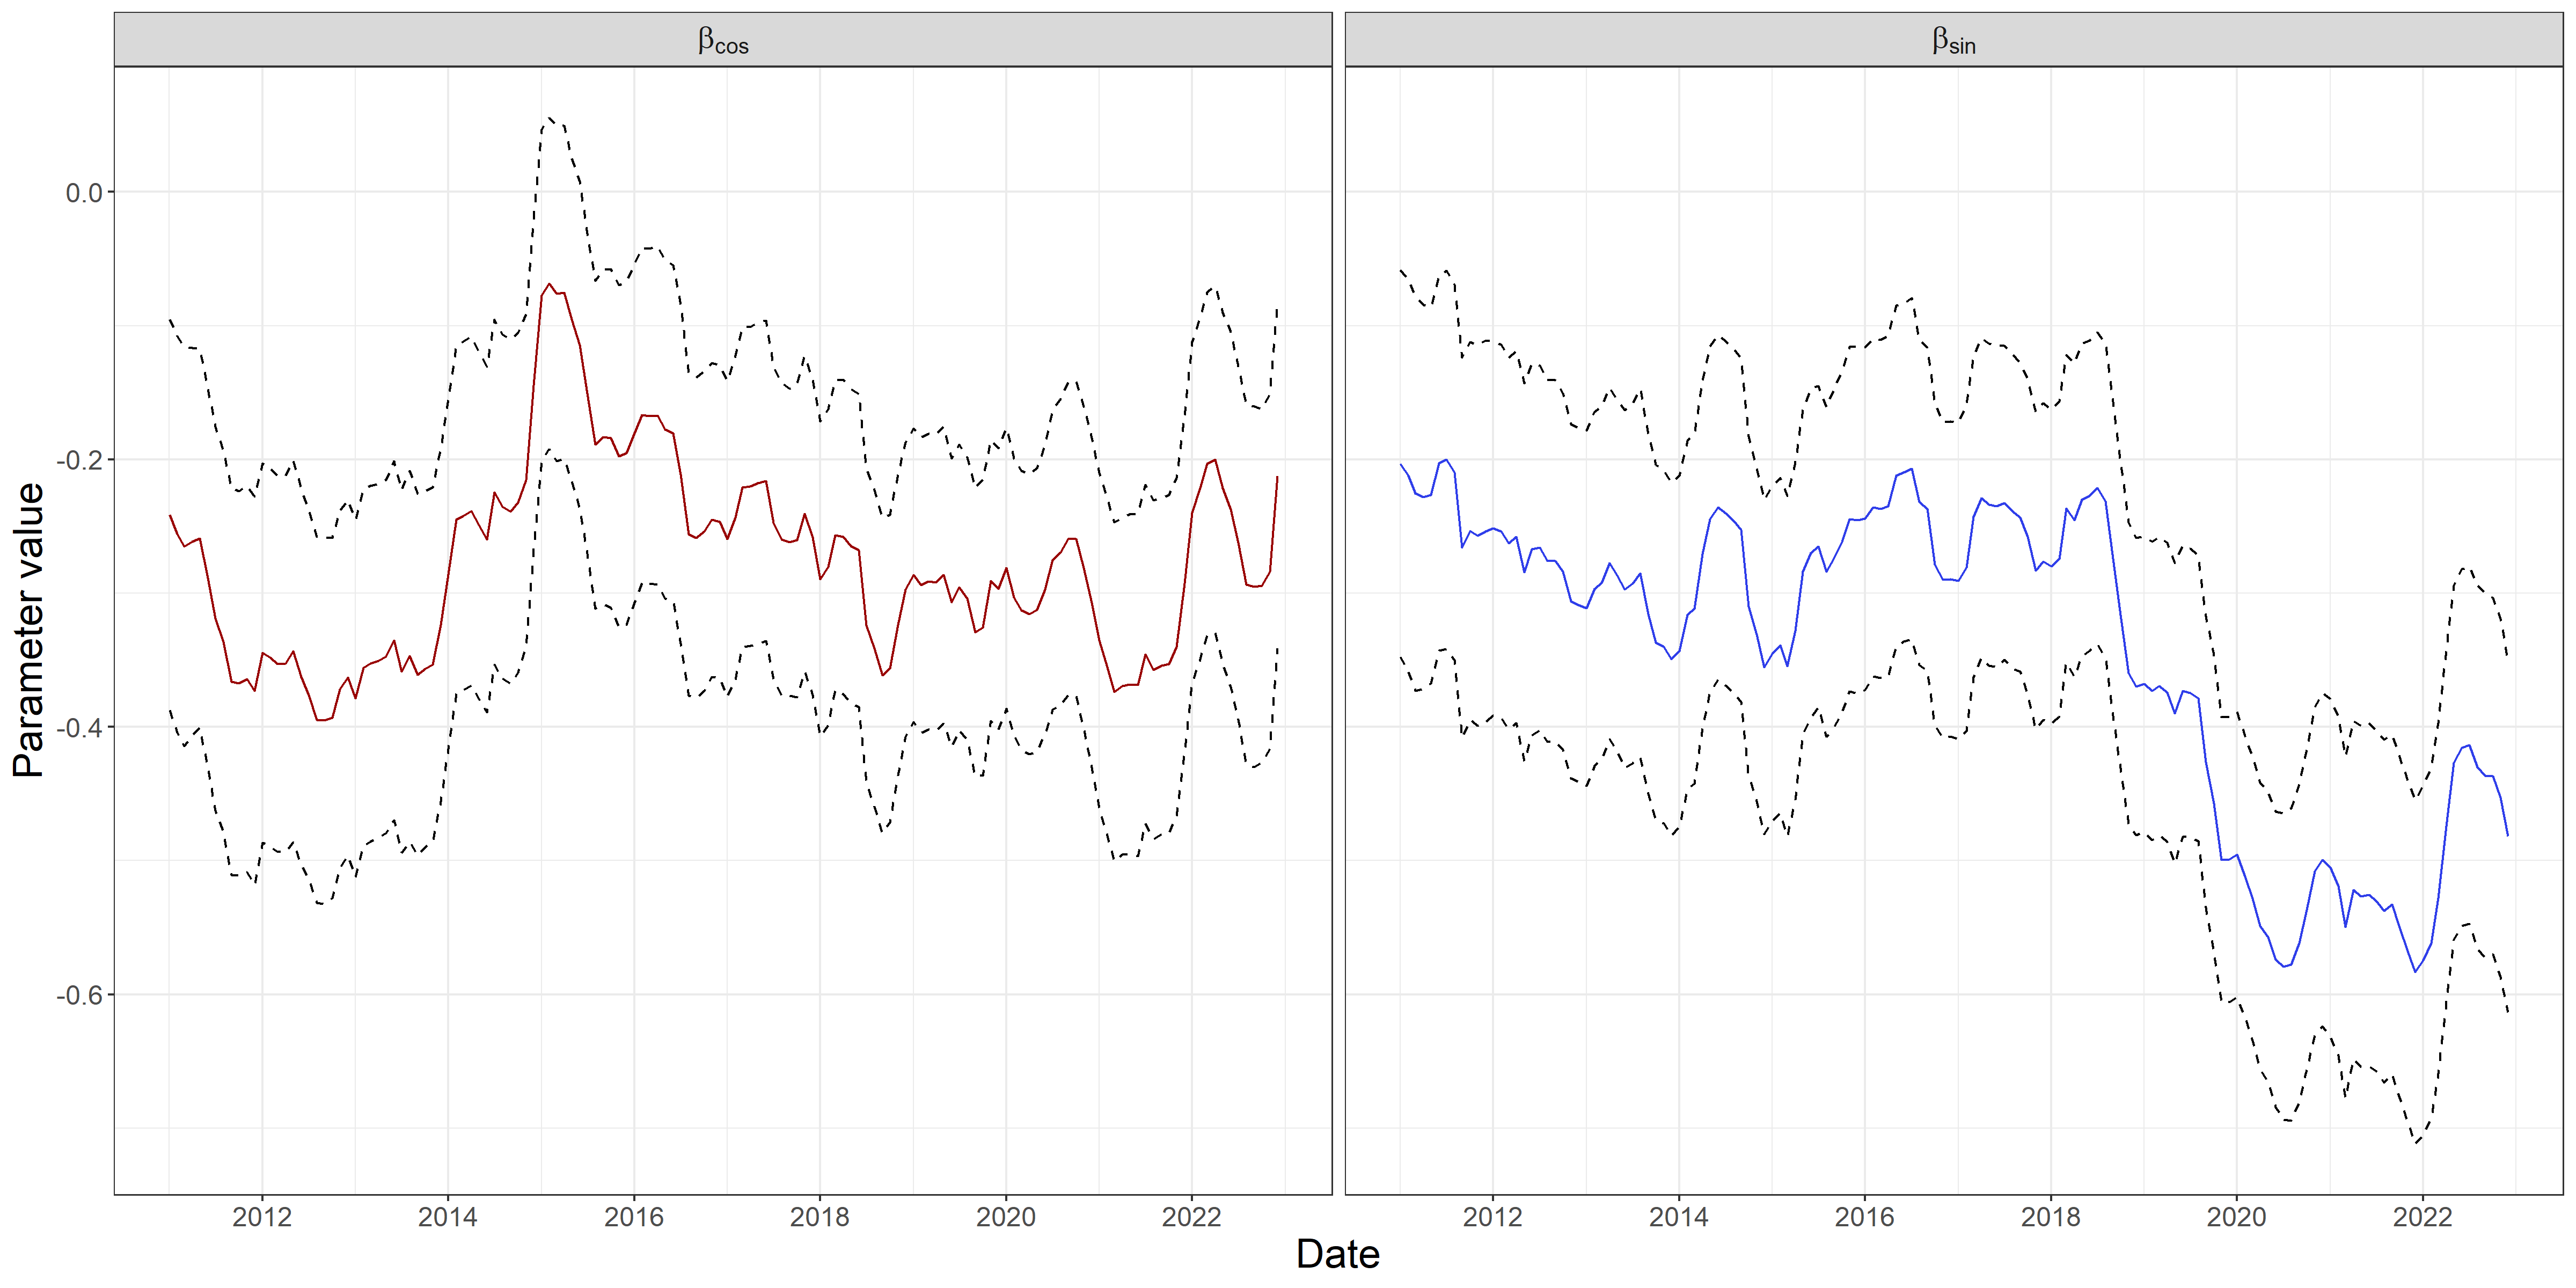
\includegraphics[width=1\linewidth]{../figures/SeasonalityParxSTEC_PoisG}

\normalsize
\end{frame}

\begin{frame}{Variance parameter}
\protect\hypertarget{variance-parameter-1}{}
\tiny

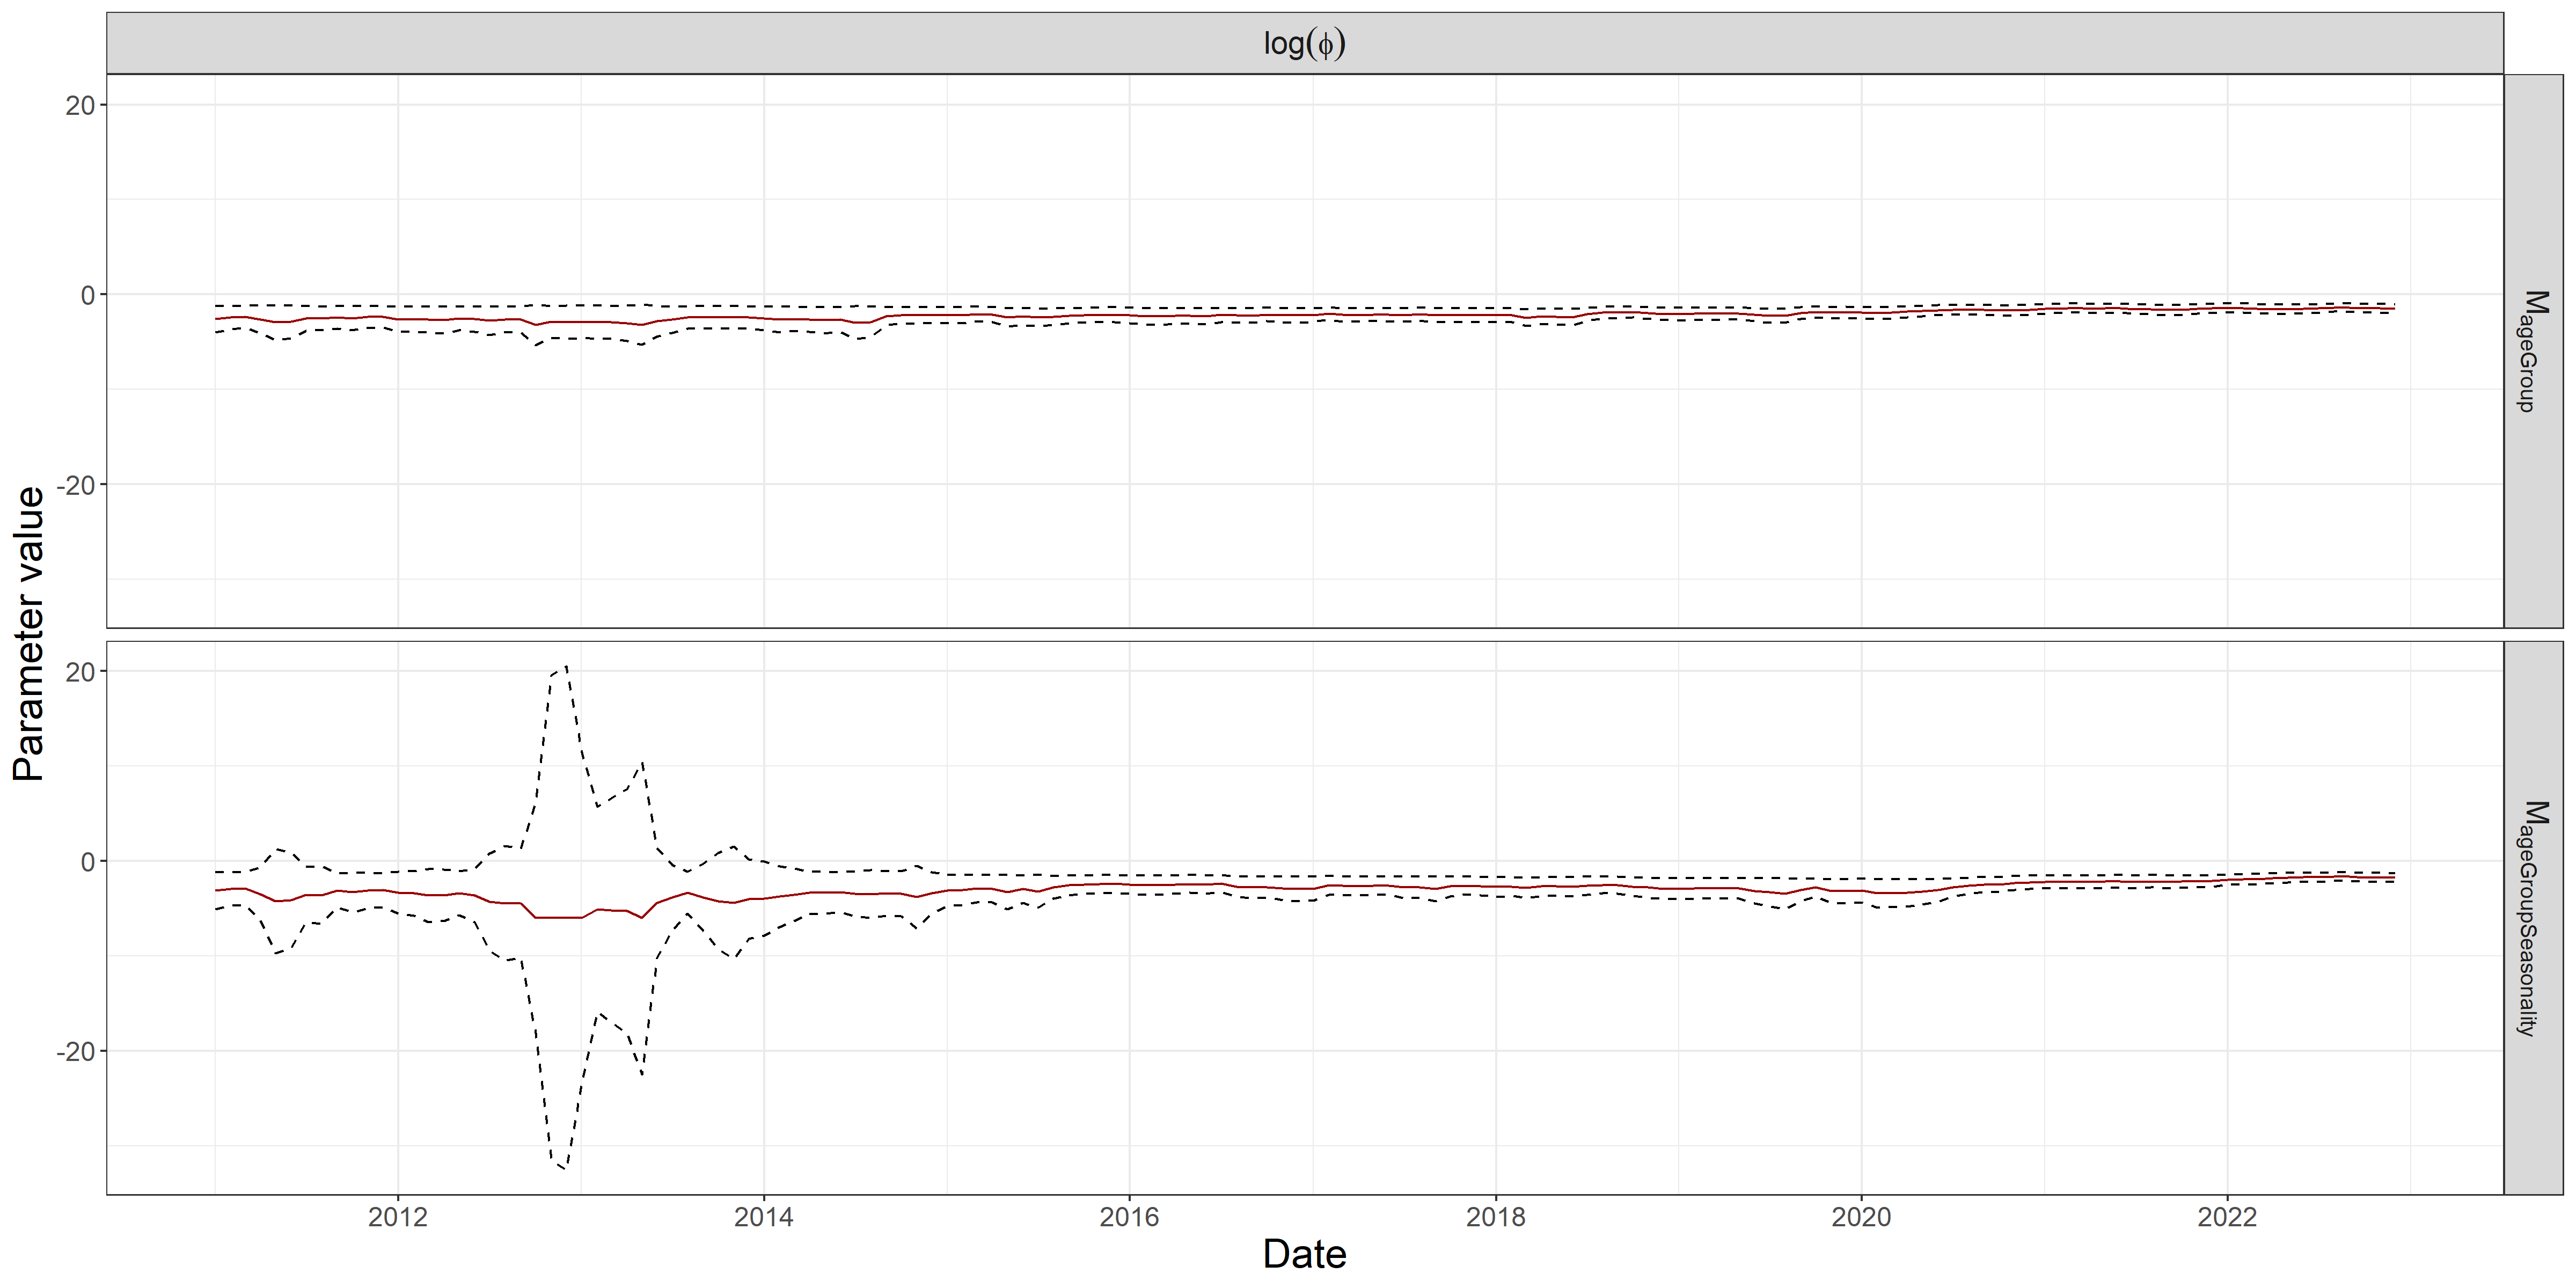
\includegraphics[width=1\linewidth]{../figures/log_phixSTEC_PoisG}

\normalsize
\end{frame}

\begin{frame}{Outbreak detection}
\protect\hypertarget{outbreak-detection-1}{}
\tiny

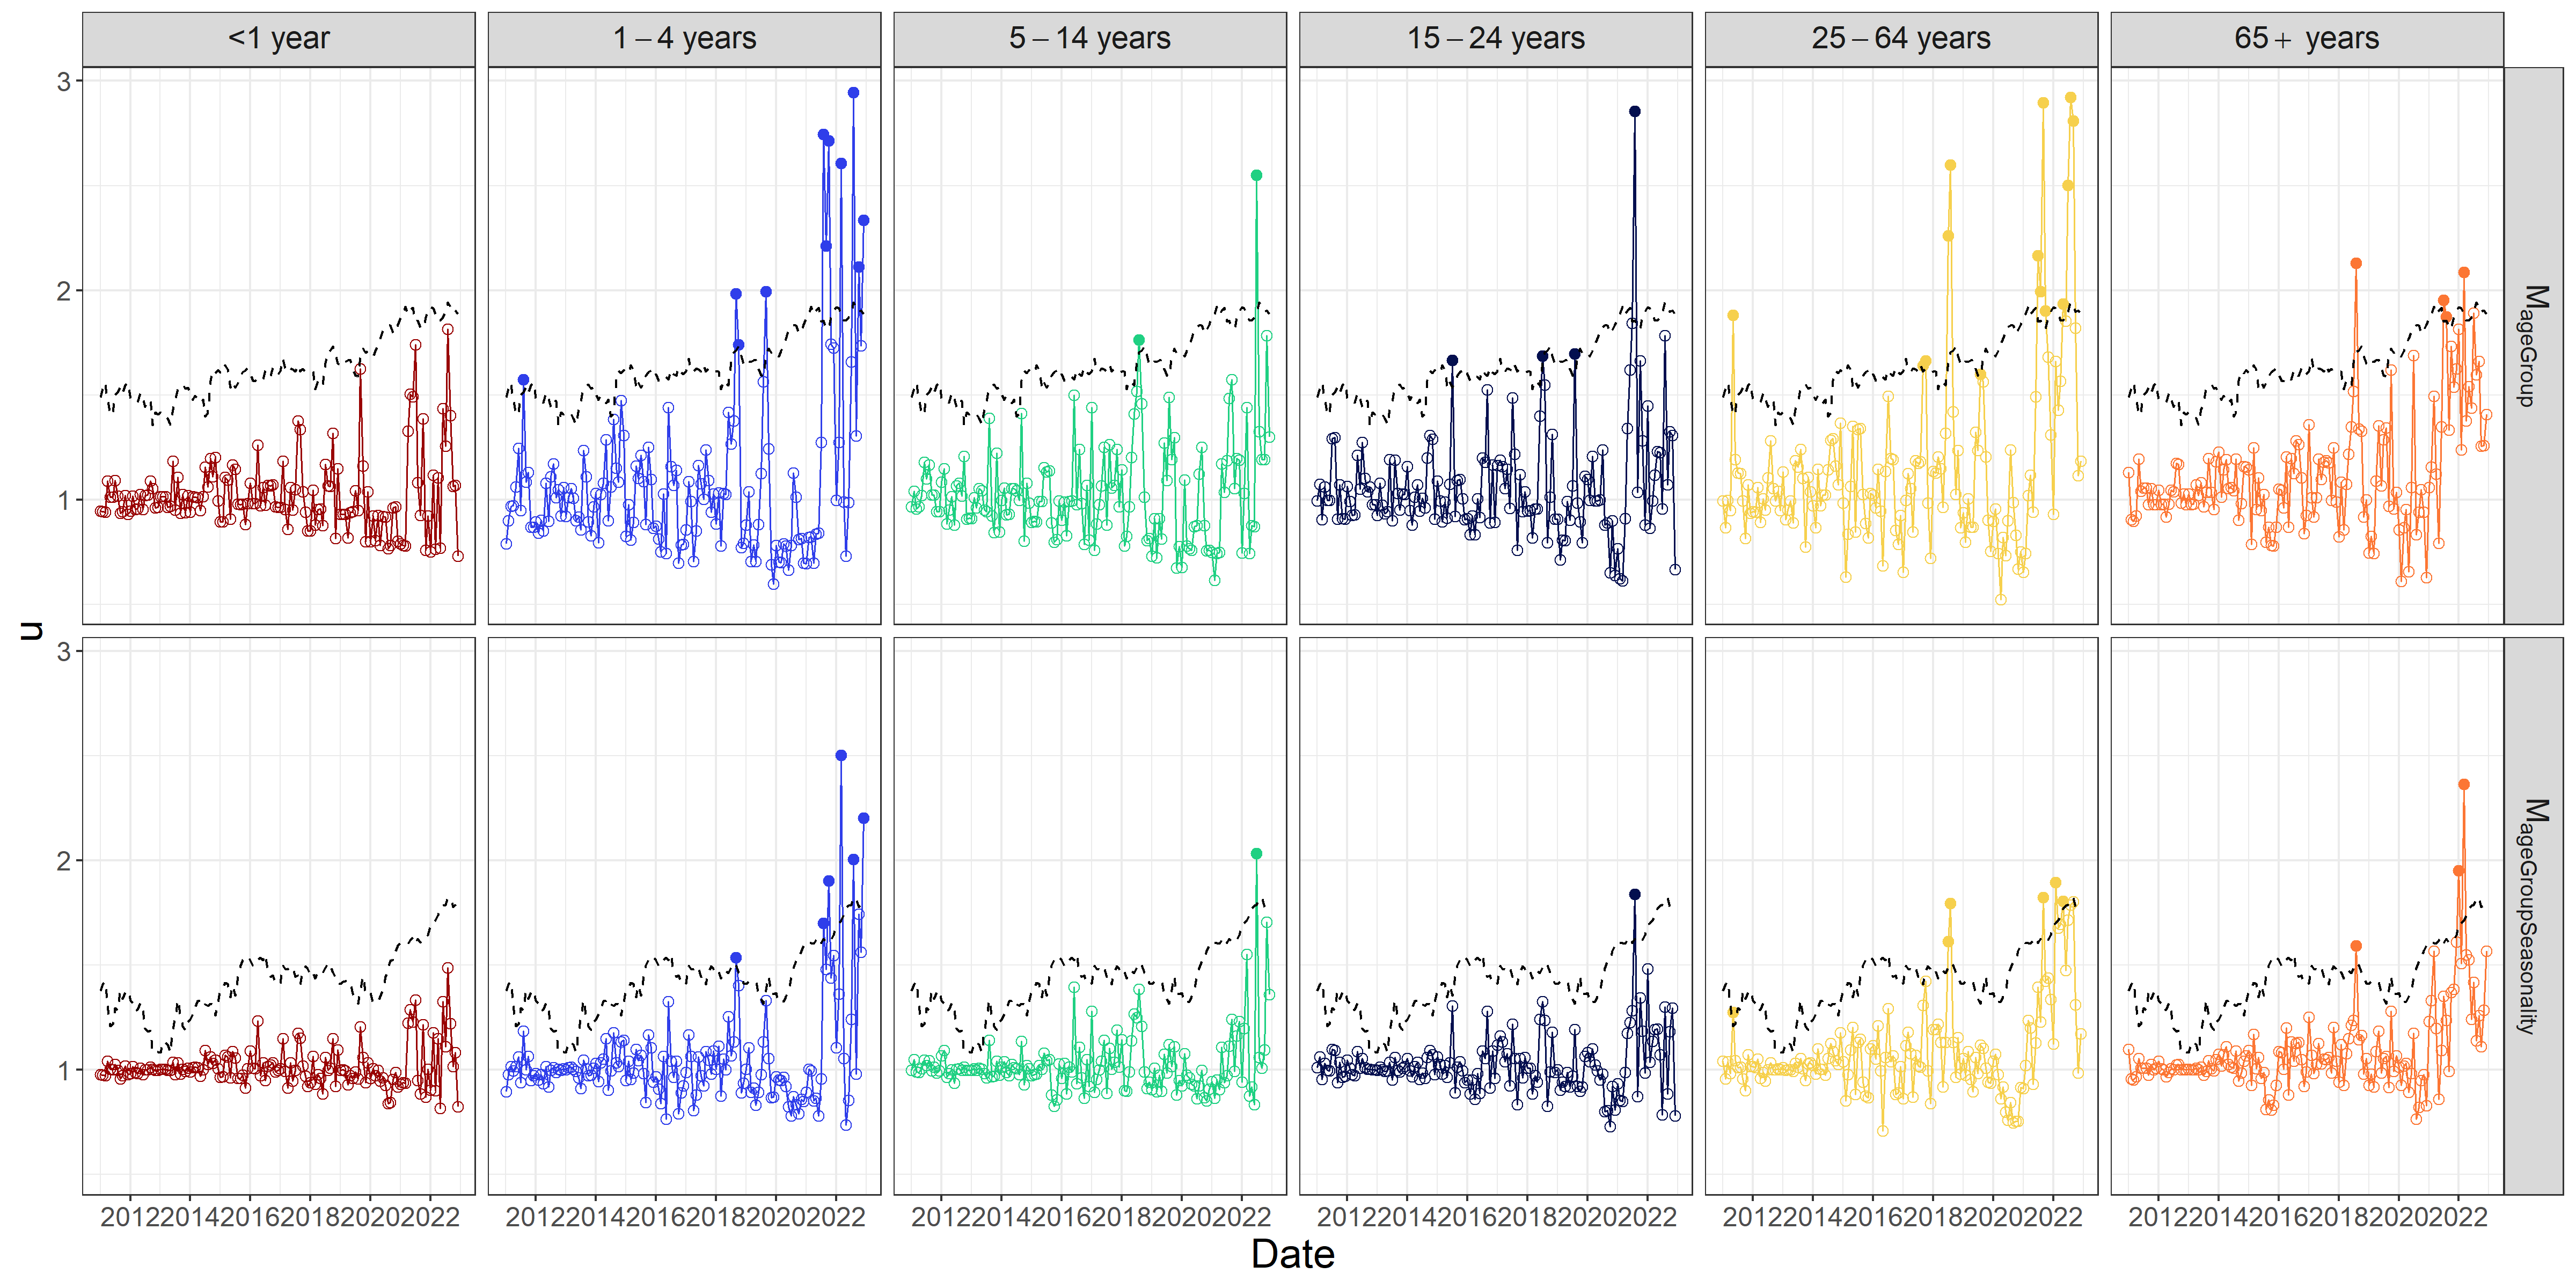
\includegraphics[width=1\linewidth]{../figures/OutbreakDetectionxSTEC_PoisG}

\normalsize
\end{frame}


\end{document}
